\chapter{Design}\label{ch:Design} %software architecture0,
The design of a robotic system for a user having a shoulder disarticulation can be quite comprehensive. this report will strive to create a proof of concept, showing that the use of a robotic limb can assist the user in a daily task.

\section{showcase}
to showcase this proof of concept, the task needing to be done has been chosen as assisting the user in drinking a cup of water.

\subsection{Equipment description}
For this project several pieces of equipment have been provided, as such the rest of this project will investigate how these can be used to accomplish our goal. the provided equipment consists of the CrustCrawler and a measuring box.

% Please add the following required packages to your document preamble:
% \usepackage{graphicx}
\begin{table}[H]
\begin{tabular}{|P{3cm}||P{10cm}|}

\hline
\textbf{Crust-Crawler} & is a robotic manipulator made by Crust-Crawler Robotics.  it consists of 5x motors capable of being mounted in a wide variation of ways.  2x Links of varying length.  these can be assembled according to the users will. \\ \hline
Moters                 & All five moters mounted on the Crust-Crawler are made by Dynamixel.  \\ \hline
Xbee S1                   & Wireless radio capable of pairing to matching device creating a "cable" \\ \hline
Teensy Board              & This is a micro controller and will work as the on board computer.      \\ \hline
Supply  board             & This board supply power from a wall plug to our system                  \\ \hline
\end{tabular}%
\caption{Description and presentation of the Crustcravler setup components}
\label{tableCrust}
\end{table}

\begin{figure}[H]
    \centering
\tikzset{every picture/.style={line width=0.75pt}} %set default line width to 0.75pt        

\begin{tikzpicture}[x=0.75pt,y=0.75pt,yscale=-1,xscale=1]
%uncomment if require: \path (0,374); %set diagram left start at 0, and has height of 374

%Image [id:dp7152221511204973] 
\draw (269.48,152.73) node  {\includegraphics[width=197.45pt,height=60.59pt]{Figures/TikzFigures/layOut/teensy.PNG}};
%Image [id:dp37486105933332636] 
\draw (366.16,279.14) node [rotate=-180.22,xslant=-0.01] {\includegraphics[width=89.36pt,height=69.95pt]{Figures/TikzFigures/layOut/supl.PNG}};
%Image [id:dp9034481830242995] 
\draw (132.79,272.76) node [rotate=-359.65,xslant=0] {\includegraphics[width=83.35pt,height=72.71pt]{Figures/TikzFigures/layOut/rs.PNG}};
%Image [id:dp11028803786694708] 
\draw (236.5,45.39) node [rotate=-270] {\includegraphics[width=60.59pt,height=62.4pt]{Figures/TikzFigures/layOut/bee.PNG}};
%Left Arrow [id:dp5012443384308891] 
\draw   (438.55,274.06) -- (457.33,256.75) -- (457.33,265.41) -- (485.5,265.41) -- (485.5,282.72) -- (457.33,282.72) -- (457.33,291.38) -- cycle ;
%Right Arrow [id:dp0023557246216043826] 
\draw   (80.2,146.67) -- (111.93,146.67) -- (111.93,137.72) -- (133.09,155.61) -- (111.93,173.5) -- (111.93,164.56) -- (80.2,164.56) -- cycle ;
%Straight Lines [id:da08227247794525927] 
\draw [color={rgb, 255:red, 247; green, 10; blue, 10 }  ,draw opacity=1 ][line width=1.5]    (150.92,81.17) -- (150.52,123.87) ;


%Straight Lines [id:da025924835708441174] 
\draw [color={rgb, 255:red, 247; green, 10; blue, 10 }  ,draw opacity=1 ][line width=1.5]    (217.48,81.17) -- (150.92,81.17) ;


%Straight Lines [id:da00602413999639384] 
\draw [color={rgb, 255:red, 247; green, 10; blue, 10 }  ,draw opacity=1 ][line width=1.5]    (42.76,80.79) -- (155.28,80.79) ;


%Straight Lines [id:da7149252935730617] 
\draw [color={rgb, 255:red, 247; green, 10; blue, 10 }  ,draw opacity=1 ][line width=1.5]    (43.55,80.79) -- (43.55,256.21) ;


%Straight Lines [id:da3829700368795059] 
\draw [color={rgb, 255:red, 247; green, 10; blue, 10 }  ,draw opacity=1 ][line width=1.5]    (91.09,256.21) -- (43.55,256.21) ;


%Straight Lines [id:da8981864779638247] 
\draw [line width=1.5]    (31.67,88.48) -- (31.67,290.84) ;


%Straight Lines [id:da6466608797084847] 
\draw [line width=1.5]    (91.89,290.07) -- (31.67,290.07) ;


%Straight Lines [id:da35185368144106244] 
\draw [line width=1.5]    (31.67,88.48) -- (272.55,89.25) ;


%Straight Lines [id:da8387196090383506] 
\draw    (271.76,80.02) -- (271.76,89.25) ;


%Straight Lines [id:da36845317589148996] 
\draw [color={rgb, 255:red, 91; green, 235; blue, 46 }  ,draw opacity=1 ][line width=1.5]    (225.01,81.56) -- (160.03,184.66) ;


%Straight Lines [id:da4171143722401429] 
\draw [color={rgb, 255:red, 248; green, 231; blue, 28 }  ,draw opacity=1 ][line width=1.5]    (231.55,81.56) -- (173.71,184.66) ;


%Straight Lines [id:da33656991606038633] 
\draw [color={rgb, 255:red, 32; green, 240; blue, 26 }  ,draw opacity=1 ][line width=1.5]    (90.3,273.91) -- (265.42,185.43) ;


%Straight Lines [id:da3740974102672152] 
\draw [color={rgb, 255:red, 244; green, 250; blue, 27 }  ,draw opacity=1 ][line width=1.5]    (255.91,184.66) -- (91.89,265.45) ;


%Straight Lines [id:da18281067478913027] 
\draw [color={rgb, 255:red, 74; green, 144; blue, 226 }  ,draw opacity=1 ][line width=1.5]    (91.09,282.37) -- (276.51,185.43) ;


%Straight Lines [id:da7137403407481466] 
\draw [line width=1.5]    (180.34,279.84) -- (343.47,319.08) ;


%Straight Lines [id:da9319303523938192] 
\draw [color={rgb, 255:red, 243; green, 20; blue, 20 }  ,draw opacity=1 ][line width=1.5]    (180.34,271.18) -- (344.5,305) ;


%Straight Lines [id:da7229658725423573] 
\draw [color={rgb, 255:red, 74; green, 144; blue, 226 }  ,draw opacity=1 ][line width=1.5]    (180.34,262.52) -- (343.5,296) ;


%Straight Lines [id:da43545523008986176] 
\draw [line width=1.5]    (31.5,202) -- (150.5,202) ;


%Straight Lines [id:da5107595655280059] 
\draw [line width=1.5]    (150.5,183) -- (150.5,202) ;



% Text Node
\draw (99.41,156.19) node  [align=left] {USB};
% Text Node
\draw (465.49,273.68) node  [align=left] {12V};
% Text Node
\draw (77,191) node  [align=left] {Gnd};
% Text Node
\draw (98,71) node  [align=left] {5V};
% Text Node
\draw (257,310) node  [align=left] {Gnd};
% Text Node
\draw (263,265) node  [align=left] {Rs 485};
% Text Node
\draw (338,106) node  [align=left] {Teensy 3.5};
% Text Node
\draw (133,341) node  [align=left] { \ \ \ BOB-10124\\Rs 232 to Rs 485};

% Text Node
\draw (212,108) node  [align=left] {Rx1 \ \ \ Tx1};
% Text Node
\draw (192,199) node  [align=left] {RxTx2};
% Text Node
\draw (317,212) node  [align=left] {Transmit enable wire};


\end{tikzpicture}
    \caption{Wiring of the Teensy to external components}
    \label{fig:motorSel}
\end{figure}
\begin{table}[H]
\begin{tabular}{|P{3cm}||P{10cm}|}
\hline
\textbf{Measurement box} & This system consists of several components housed in a 3X printed box   \\ \hline
XBee S1                  & Wireless radio capable of pairing to matching device creating a "cable" \\ \hline
Battery                  & type CR123A, normally used for cameras                                  \\ \hline
5x Inputs                & 2 x Sparkfun EMG boards + 3 axis Accelerometer                         \\ \hline
\end{tabular}%
\caption{Description of components in the measurement box}
\label{tableBOX}
\end{table}
\section{Data flow}
The figure below shows the data flow of the solution presented in this chapter. A single line in the arrow signifies that data is flowing one way and a double line means that information is both being sent and received.
\begin{figure}[H]
    \centering
    

\tikzset{every picture/.style={line width=0.75pt}} %set default line width to 0.75pt        

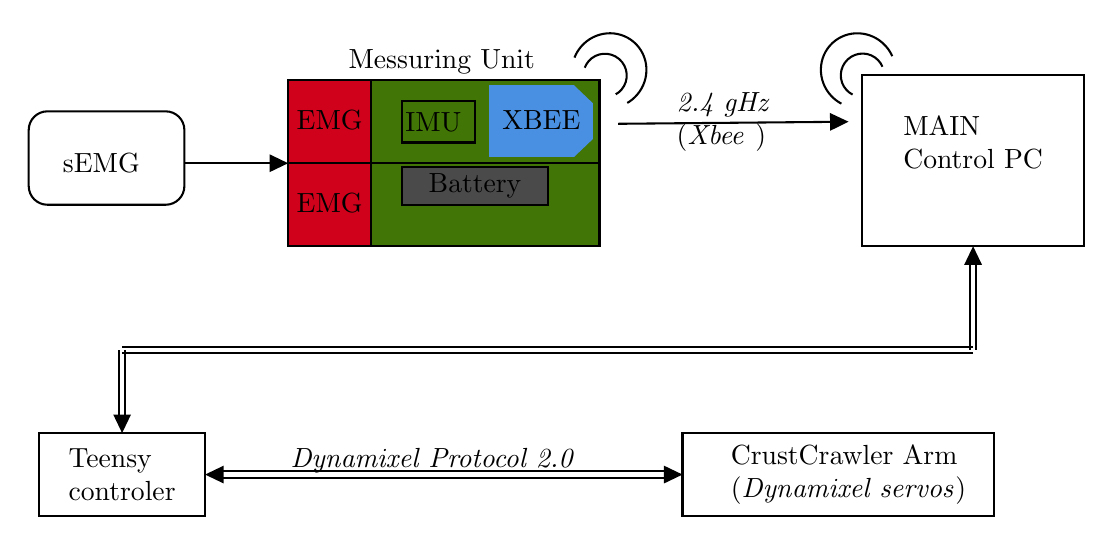
\begin{tikzpicture}[x=0.75pt,y=0.75pt,yscale=-1,xscale=1]
%uncomment if require: \path (0,278.7142848968506); %set diagram left start at 0, and has height of 278.7142848968506

%Shape: Rectangle [id:dp9058146125823148] 
\draw   (436.69,27.6) -- (543.37,27.6) -- (543.37,110) -- (436.69,110) -- cycle ;
%Rounded Rect [id:dp9198394438295476] 
\draw   (35,54) .. controls (35,49.03) and (39.03,45) .. (44,45) -- (101,45) .. controls (105.97,45) and (110,49.03) .. (110,54) -- (110,81) .. controls (110,85.97) and (105.97,90) .. (101,90) -- (44,90) .. controls (39.03,90) and (35,85.97) .. (35,81) -- cycle ;
%Straight Lines [id:da08300314610956905] 
\draw    (110,70) -- (158,70) ;
\draw [shift={(160,70)}, rotate = 180] [fill={rgb, 255:red, 0; green, 0; blue, 0 }  ][line width=0.75]  [draw opacity=0] (8.93,-4.29) -- (0,0) -- (8.93,4.29) -- cycle    ;

%Shape: Rectangle [id:dp49994760485296896] 
\draw  [fill={rgb, 255:red, 65; green, 117; blue, 5 }  ,fill opacity=1 ] (160,30) -- (310,30) -- (310,110) -- (160,110) -- cycle ;
%Shape: Rectangle [id:dp9990642544965083] 
\draw  [fill={rgb, 255:red, 208; green, 2; blue, 27 }  ,fill opacity=1 ] (160,30) -- (200,30) -- (200,70) -- (160,70) -- cycle ;
%Shape: Rectangle [id:dp5155575250253981] 
\draw  [fill={rgb, 255:red, 208; green, 2; blue, 27 }  ,fill opacity=1 ] (160,70) -- (200,70) -- (200,110) -- (160,110) -- cycle ;
%Straight Lines [id:da2266079205645528] 
\draw    (319,51) -- (428,50.02) ;
\draw [shift={(430,50)}, rotate = 539.48] [fill={rgb, 255:red, 0; green, 0; blue, 0 }  ][line width=0.75]  [draw opacity=0] (8.93,-4.29) -- (0,0) -- (8.93,4.29) -- cycle    ;

%Shape: Rectangle [id:dp7097032559017205] 
\draw  [fill={rgb, 255:red, 65; green, 117; blue, 5 }  ,fill opacity=1 ] (200,30) -- (310,30) -- (310,70) -- (200,70) -- cycle ;
%Shape: Rectangle [id:dp16739603109917534] 
\draw  [fill={rgb, 255:red, 65; green, 117; blue, 5 }  ,fill opacity=1 ] (200,70) -- (310,70) -- (310,110) -- (200,110) -- cycle ;
%Shape: Diagonal Stripe [id:dp825501516378429] 
\draw  [color={rgb, 255:red, 0; green, 0; blue, 0 }  ,draw opacity=0 ][fill={rgb, 255:red, 74; green, 144; blue, 226 }  ,fill opacity=1 ] (306.79,58.36) -- (297.73,67) -- (297.73,32.43) -- (306.79,41.07) -- cycle ;
%Shape: Rectangle [id:dp443446878421101] 
\draw  [draw opacity=0][fill={rgb, 255:red, 74; green, 144; blue, 226 }  ,fill opacity=1 ] (257,32.43) -- (297.73,32.43) -- (297.73,67) -- (257,67) -- cycle ;

%Shape: Rectangle [id:dp7890442898232035] 
\draw  [fill={rgb, 255:red, 74; green, 74; blue, 74 }  ,fill opacity=1 ] (215,72) -- (285,72) -- (285,90) -- (215,90) -- cycle ;
%Shape: Rectangle [id:dp3185767197775584] 
\draw  [fill={rgb, 255:red, 65; green, 117; blue, 5 }  ,fill opacity=1 ] (215,40) -- (250,40) -- (250,60) -- (215,60) -- cycle ;
%Shape: Arc [id:dp6014275798651711] 
\draw  [draw opacity=0] (302.89,23.99) .. controls (303.31,22.88) and (303.92,21.82) .. (304.74,20.86) .. controls (308.48,16.5) and (315.08,16.02) .. (319.46,19.79) .. controls (323.85,23.55) and (324.37,30.14) .. (320.63,34.5) .. controls (319.81,35.46) and (318.86,36.23) .. (317.82,36.8) -- (312.69,27.68) -- cycle ; \draw   (302.89,23.99) .. controls (303.31,22.88) and (303.92,21.82) .. (304.74,20.86) .. controls (308.48,16.5) and (315.08,16.02) .. (319.46,19.79) .. controls (323.85,23.55) and (324.37,30.14) .. (320.63,34.5) .. controls (319.81,35.46) and (318.86,36.23) .. (317.82,36.8) ;
%Shape: Arc [id:dp584505117797834] 
\draw  [draw opacity=0] (297.95,19.11) .. controls (298.69,17.23) and (299.75,15.44) .. (301.14,13.82) .. controls (307.69,6.19) and (319.05,5.19) .. (326.5,11.59) .. controls (333.96,17.98) and (334.69,29.36) .. (328.14,36.99) .. controls (326.75,38.61) and (325.14,39.94) .. (323.39,40.95) -- (314.64,25.4) -- cycle ; \draw   (297.95,19.11) .. controls (298.69,17.23) and (299.75,15.44) .. (301.14,13.82) .. controls (307.69,6.19) and (319.05,5.19) .. (326.5,11.59) .. controls (333.96,17.98) and (334.69,29.36) .. (328.14,36.99) .. controls (326.75,38.61) and (325.14,39.94) .. (323.39,40.95) ;

%Shape: Arc [id:dp9643215893864674] 
\draw  [draw opacity=0] (431.94,36.92) .. controls (430.88,36.39) and (429.9,35.66) .. (429.04,34.74) .. controls (425.12,30.54) and (425.37,23.93) .. (429.6,19.99) .. controls (433.82,16.04) and (440.43,16.25) .. (444.35,20.46) .. controls (445.21,21.38) and (445.87,22.41) .. (446.33,23.51) -- (436.69,27.6) -- cycle ; \draw   (431.94,36.92) .. controls (430.88,36.39) and (429.9,35.66) .. (429.04,34.74) .. controls (425.12,30.54) and (425.37,23.93) .. (429.6,19.99) .. controls (433.82,16.04) and (440.43,16.25) .. (444.35,20.46) .. controls (445.21,21.38) and (445.87,22.41) .. (446.33,23.51) ;
%Shape: Arc [id:dp6589182805450249] 
\draw  [draw opacity=0] (426.55,41.3) .. controls (424.76,40.36) and (423.1,39.1) .. (421.64,37.54) .. controls (414.78,30.18) and (415.04,18.79) .. (422.22,12.09) .. controls (429.41,5.39) and (440.79,5.91) .. (447.65,13.27) .. controls (449.11,14.83) and (450.25,16.58) .. (451.07,18.43) -- (434.64,25.4) -- cycle ; \draw   (426.55,41.3) .. controls (424.76,40.36) and (423.1,39.1) .. (421.64,37.54) .. controls (414.78,30.18) and (415.04,18.79) .. (422.22,12.09) .. controls (429.41,5.39) and (440.79,5.91) .. (447.65,13.27) .. controls (449.11,14.83) and (450.25,16.58) .. (451.07,18.43) ;

%Straight Lines [id:da8446148813559833] 
\draw    (491.5,118) -- (491.5,160)(488.5,118) -- (488.5,160) ;

\draw [shift={(490,110)}, rotate = 90] [fill={rgb, 255:red, 0; green, 0; blue, 0 }  ][line width=0.75]  [draw opacity=0] (8.93,-4.29) -- (0,0) -- (8.93,4.29) -- cycle    ;
%Straight Lines [id:da5044267925519024] 
\draw    (490,161.5) -- (80,161.5)(490,158.5) -- (80,158.5) ;


%Straight Lines [id:da7406026285596496] 
\draw    (81.5,160) -- (81.5,192)(78.5,160) -- (78.5,192) ;
\draw [shift={(80,200)}, rotate = 270] [fill={rgb, 255:red, 0; green, 0; blue, 0 }  ][line width=0.75]  [draw opacity=0] (8.93,-4.29) -- (0,0) -- (8.93,4.29) -- cycle    ;

%Shape: Rectangle [id:dp016623272212034745] 
\draw   (40,200) -- (120,200) -- (120,240) -- (40,240) -- cycle ;
%Straight Lines [id:da7263406511929] 
\draw    (128,218.5) -- (342,218.5)(128,221.5) -- (342,221.5) ;
\draw [shift={(350,220)}, rotate = 180] [fill={rgb, 255:red, 0; green, 0; blue, 0 }  ][line width=0.75]  [draw opacity=0] (8.93,-4.29) -- (0,0) -- (8.93,4.29) -- cycle    ;
\draw [shift={(120,220)}, rotate = 0] [fill={rgb, 255:red, 0; green, 0; blue, 0 }  ][line width=0.75]  [draw opacity=0] (8.93,-4.29) -- (0,0) -- (8.93,4.29) -- cycle    ;
%Shape: Rectangle [id:dp6457555540924869] 
\draw   (350,200) -- (500,200) -- (500,240) -- (350,240) -- cycle ;

% Text Node
\draw (490,60) node  [align=left] {MAIN\\Control PC};
% Text Node
\draw (70,70) node  [align=left] {sEMG};
% Text Node
\draw (234,21) node  [align=left] {Messuring Unit};
% Text Node
\draw (282,49) node  [align=left] {XBEE};
% Text Node
\draw (370,50) node  [align=left] {\textit{2.4 gHz}\\(\textit{Xbee })};
% Text Node
\draw (250,81) node  [align=left] {Battery};
% Text Node
\draw (180,49) node  [align=left] {EMG};
% Text Node
\draw (180,89) node  [align=left] {EMG};
% Text Node
\draw (230,50) node  [align=left] {IMU};
% Text Node
\draw (80,220) node  [align=left] {Teensy\\controler};
% Text Node
\draw (230,220) node  [align=left] {\textit{Dynamixel Protocol 2.0}\\};
% Text Node
\draw (430,220) node  [align=left] {CrustCrawler Arm\\(\textit{Dynamixel servos})};


\end{tikzpicture}

    \caption{Data flowchart}
    \label{fig:DataFlow}
\end{figure}
\subsection{Measuring unit}
On the user, a grey measuring box is mounted. This box consists of two Sparkfun Muscle Sensor Platinum V3.3 EMG sensors, one Polulo 3-Axis Accelerometer, a battery and an XBee S1 radio module.
\subsubsection{Sparkfun EMG sensors}
The sensor measures raw EMG, however, this is not what is received by the rest of the system. First, the raw data is sent through a circuit that rectifies the raw EMG this means taking the root square of the input in order only to have positive data. After this, a small number of data points is then summed and averaged to smooth the data out in the smooth circuit. After the rectification and smoothing the data is sent to the XBee. A full schematic of the EMG sensors can be seen in Appendix \ref{app:EMGsensor}
\subsubsection{Polulo Accelerometer}
This is a simple 3-axis accelerometer providing further 3 channels of input into the measuring box. 
\subsubsection{Wireless transition with Xbee}\label{XbeeExplan}
The XBee S1 radio module is the foundation of the wireless transmission of data in this solution. It has a frequency of $100Hz$ and sends a frame on every sample which is created every $0.10s$ and the frame consists of 24 bytes. The structure of the 24 bytes can be seen below in figure \ref{fig:XbeeFrame}
\begin{figure}[H]
    \centering
    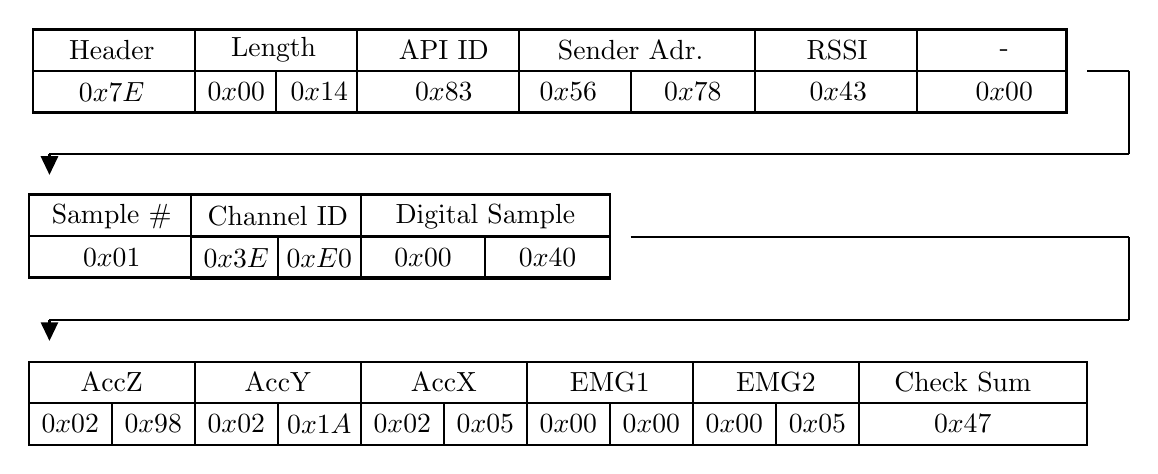
\begin{tikzpicture}[x=0.75pt,y=0.75pt,yscale=-1,xscale=1]
%uncomment if require: \path (0,230.14285278320312); %set diagram left start at 0, and has height of 230.14285278320312

%Shape: Rectangle [id:dp10856467985503815] 
\draw   (22,10) -- (520,10) -- (520,50) -- (22,50) -- cycle ;
%Shape: Rectangle [id:dp1921303622580388] 
\draw   (22,10) -- (100,10) -- (100,30) -- (22,30) -- cycle ;
%Shape: Rectangle [id:dp5511536446299157] 
\draw   (22,30) -- (100,30) -- (100,50) -- (22,50) -- cycle ;
%Shape: Rectangle [id:dp8551124842169571] 
\draw   (100,30) -- (178,30) -- (178,50) -- (100,50) -- cycle ;
%Shape: Rectangle [id:dp1542301721460031] 
\draw   (100,10) -- (178,10) -- (178,30) -- (100,30) -- cycle ;
%Shape: Rectangle [id:dp39637490877675896] 
\draw   (100,30) -- (139,30) -- (139,50) -- (100,50) -- cycle ;
%Shape: Rectangle [id:dp7008641367286479] 
\draw   (178,10) -- (256,10) -- (256,30) -- (178,30) -- cycle ;
%Shape: Rectangle [id:dp6311822380704302] 
\draw   (178,30) -- (256,30) -- (256,50) -- (178,50) -- cycle ;
%Shape: Rectangle [id:dp2794130706147937] 
\draw   (256,10) -- (370,10) -- (370,30) -- (256,30) -- cycle ;
%Shape: Rectangle [id:dp0748834298647747] 
\draw   (256,30) -- (370,30) -- (370,50) -- (256,50) -- cycle ;
%Shape: Rectangle [id:dp3442757233060003] 
\draw   (256,30) -- (310,30) -- (310,50) -- (256,50) -- cycle ;
%Shape: Rectangle [id:dp7243088972581471] 
\draw   (370,10) -- (448,10) -- (448,30) -- (370,30) -- cycle ;
%Shape: Rectangle [id:dp8634226198686377] 
\draw   (370,30) -- (448,30) -- (448,50) -- (370,50) -- cycle ;
%Shape: Rectangle [id:dp049451176775102246] 
\draw   (448,30) -- (520,30) -- (520,50) -- (448,50) -- cycle ;
%Shape: Rectangle [id:dp10185955763756471] 
\draw   (448,10) -- (520,10) -- (520,30) -- (448,30) -- cycle ;
%Shape: Rectangle [id:dp3116685664620873] 
\draw   (20,89.5) -- (300,89.5) -- (300,129.5) -- (20,129.5) -- cycle ;
%Shape: Rectangle [id:dp4024383934360989] 
\draw   (20,89.5) -- (98,89.5) -- (98,109.5) -- (20,109.5) -- cycle ;
%Shape: Rectangle [id:dp9664793454969085] 
\draw   (20,109.5) -- (98,109.5) -- (98,129.5) -- (20,129.5) -- cycle ;
%Shape: Rectangle [id:dp4124508293977984] 
\draw   (98,109.5) -- (180,109.5) -- (180,129.5) -- (98,129.5) -- cycle ;
%Shape: Rectangle [id:dp711781414287457] 
\draw   (98,89.5) -- (180,89.5) -- (180,110) -- (98,110) -- cycle ;
%Shape: Rectangle [id:dp356328253424953] 
\draw   (98,110) -- (140,110) -- (140,130) -- (98,130) -- cycle ;
%Shape: Rectangle [id:dp6733077815498894] 
\draw   (180,89.5) -- (300,89.5) -- (300,110) -- (180,110) -- cycle ;
%Shape: Rectangle [id:dp6479637887159722] 
\draw   (180,109.5) -- (300,109.5) -- (300,130) -- (180,130) -- cycle ;
%Shape: Rectangle [id:dp19346515996870206] 
\draw   (180,110) -- (240,110) -- (240,130) -- (180,130) -- cycle ;
%Shape: Rectangle [id:dp38146177317207886] 
\draw   (20,170) -- (530,170) -- (530,210) -- (20,210) -- cycle ;
%Shape: Rectangle [id:dp4556101293933754] 
\draw   (20,170) -- (100,170) -- (100,190) -- (20,190) -- cycle ;
%Shape: Rectangle [id:dp5407175554825892] 
\draw   (20,190) -- (60,190) -- (60,210) -- (20,210) -- cycle ;
%Shape: Rectangle [id:dp7450461679704352] 
\draw   (60,190) -- (100,190) -- (100,210) -- (60,210) -- cycle ;
%Shape: Rectangle [id:dp4332754864269053] 
\draw   (100,170) -- (180,170) -- (180,190) -- (100,190) -- cycle ;
%Shape: Rectangle [id:dp28452698286293754] 
\draw   (140,190) -- (180,190) -- (180,210) -- (140,210) -- cycle ;
%Shape: Rectangle [id:dp7914115317030024] 
\draw   (100,190) -- (140,190) -- (140,210) -- (100,210) -- cycle ;
%Shape: Rectangle [id:dp38727788354631554] 
\draw   (220,190) -- (260,190) -- (260,210) -- (220,210) -- cycle ;
%Shape: Rectangle [id:dp22288528455712386] 
\draw   (180,190) -- (220,190) -- (220,210) -- (180,210) -- cycle ;
%Shape: Rectangle [id:dp8165391393896375] 
\draw   (180,170) -- (260,170) -- (260,190) -- (180,190) -- cycle ;
%Shape: Rectangle [id:dp6523955550843537] 
\draw   (260,190) -- (300,190) -- (300,210) -- (260,210) -- cycle ;
%Shape: Rectangle [id:dp9747757771531758] 
\draw   (300,190) -- (340,190) -- (340,210) -- (300,210) -- cycle ;
%Shape: Rectangle [id:dp8745951425419776] 
\draw   (260,170) -- (340,170) -- (340,190) -- (260,190) -- cycle ;
%Shape: Rectangle [id:dp9793885365492223] 
\draw   (340,170) -- (420,170) -- (420,190) -- (340,190) -- cycle ;
%Shape: Rectangle [id:dp03157812028724449] 
\draw   (340,190) -- (380,190) -- (380,210) -- (340,210) -- cycle ;
%Shape: Rectangle [id:dp24057366681022452] 
\draw   (380,190) -- (420,190) -- (420,210) -- (380,210) -- cycle ;
%Shape: Rectangle [id:dp36093082441092617] 
\draw   (140,110) -- (180,110) -- (180,130) -- (140,130) -- cycle ;
%Shape: Rectangle [id:dp7171363093153074] 
\draw   (420,170) -- (530,170) -- (530,190) -- (420,190) -- cycle ;
%Shape: Rectangle [id:dp5647098232631986] 
\draw   (420,190) -- (530,190) -- (530,210) -- (420,210) -- cycle ;
%Straight Lines [id:da6332689457085323] 
\draw    (530,30) -- (550,30) ;


%Straight Lines [id:da30561509563968503] 
\draw    (550,30) -- (550,70) ;


%Straight Lines [id:da09566559311573841] 
\draw    (550,70) -- (30,70) ;


%Straight Lines [id:da5601518731242143] 
\draw    (30,70) -- (30,78) ;
\draw [shift={(30,80)}, rotate = 270] [fill={rgb, 255:red, 0; green, 0; blue, 0 }  ][line width=0.75]  [draw opacity=0] (8.93,-4.29) -- (0,0) -- (8.93,4.29) -- cycle    ;

%Straight Lines [id:da9169109459317539] 
\draw    (310,110) -- (550,110) ;


%Straight Lines [id:da5912944234587121] 
\draw    (550,110) -- (550,150) ;


%Straight Lines [id:da7375405804531086] 
\draw    (550,150) -- (30,150) ;


%Straight Lines [id:da024754719673693026] 
\draw    (30,150) -- (30,158) ;
\draw [shift={(30,160)}, rotate = 270] [fill={rgb, 255:red, 0; green, 0; blue, 0 }  ][line width=0.75]  [draw opacity=0] (8.93,-4.29) -- (0,0) -- (8.93,4.29) -- cycle    ;


% Text Node
\draw (60,20) node  [align=left] {Header};
% Text Node
\draw (60,40) node   {$0x7E$};
% Text Node
\draw (138,19.5) node  [align=left] {Length};
% Text Node
\draw (120,40) node   {$0x00$};
% Text Node
\draw (160,40) node   {$0x14$};
% Text Node
\draw (220,20) node  [align=left] {API ID};
% Text Node
\draw (220,40) node   {$0x83$};
% Text Node
\draw (310,20) node  [align=left] {Sender Adr.};
% Text Node
\draw (280,40) node   {$0x56$};
% Text Node
\draw (340,40) node   {$0x78$};
% Text Node
\draw (409.5,20) node  [align=left] {RSSI};
% Text Node
\draw (410,40) node   {$0x43$};
% Text Node
\draw (490,20) node  [align=left] {\mbox{-}};
% Text Node
\draw (490,40) node   {$0x00$};
% Text Node
\draw (60,100) node  [align=left] {Sample \#};
% Text Node
\draw (60,120) node   {$0x01$};
% Text Node
\draw (140,100) node  [align=left] {Channel ID};
% Text Node
\draw (120,120) node   {$0x3E$};
% Text Node
\draw (160,120) node   {$0xE0$};
% Text Node
\draw (240,100) node  [align=left] {Digital Sample};
% Text Node
\draw (210,120) node   {$0x00$};
% Text Node
\draw (270,120) node   {$0x40$};
% Text Node
\draw (60,180) node  [align=left] {AccZ};
% Text Node
\draw (40,200) node   {$0x02$};
% Text Node
\draw (80,200) node   {$0x98$};
% Text Node
\draw (140,180) node  [align=left] {AccY};
% Text Node
\draw (120,200) node   {$0x02$};
% Text Node
\draw (160,200) node   {$0x1A$};
% Text Node
\draw (220,180) node  [align=left] {AccX};
% Text Node
\draw (200,200) node   {$0x02$};
% Text Node
\draw (240,200) node   {$0x05$};
% Text Node
\draw (280,200) node   {$0x00$};
% Text Node
\draw (320,200) node   {$0x00$};
% Text Node
\draw (300,180) node  [align=left] {EMG1};
% Text Node
\draw (360,200) node   {$0x00$};
% Text Node
\draw (400,200) node   {$0x05$};
% Text Node
\draw (380,180) node  [align=left] {EMG2};
% Text Node
\draw (470,180) node  [align=left] {Check Sum};
% Text Node
\draw (470,200) node   {$0x47$};


\end{tikzpicture}

    \caption{XBee Frame arrows indicate the direction to read.}
    \label{fig:XbeeFrame}
\end{figure}\label{XbeeDataStruct}
The first is the header-byte, this determines the start of a new frame, after that there is the information on the length of the frame. This checks if all 24 bytes are in the frame. Afterwards, there is information on the XBee module followed by data gathered from the sensors and is ended by the CheckSum that checks if the data is transferred correctly.
\subsection{Main Control PC}
The Main Control PC (MCP) receive information from the measuring unit and the robot. The measuring unit data is converted into an output that is readable to the robot.
\subsubsection{Dynamixel Protocol 2.0}
The Dynamixel Servos is communicated with via the Dynamixel Protocol 2.0.
The communication of the Dynamixelmotors on the robot arm has is a modular and daisy-chained system that supports data packet control. The packets consist of two parts. An instructional packet is sent to the motors, and a status packet is received from the motors. 

\missingfigure{CAN BE SEEN HERE \label{fig:DynamixelStructure} \url{http://www.robotis.us/product_images/uploaded_images/dynamixel-03-2012.jpg}}

As seen in figure \ref{fig:DynamixelStructure} above is the data structure on the Dynamixel servos. A header determining the start off the packet and direction information, and a payload where most of the information is stored. 
\paragraph{The instructional packet} has the basic structure seen the the figure bellow:
\begin{figure}[H]
    \centering
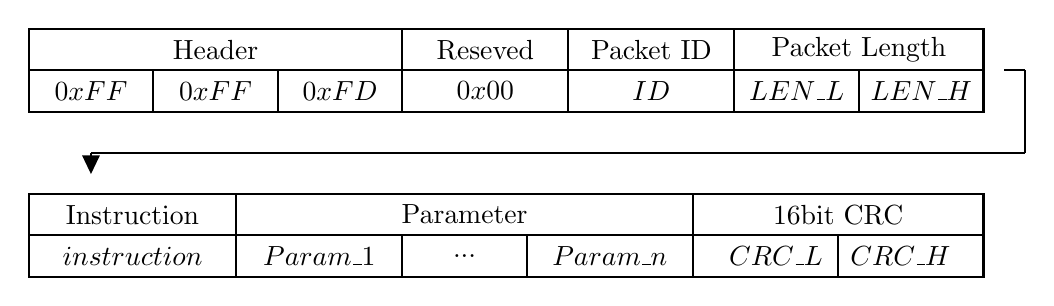
\begin{tikzpicture}[x=0.75pt,y=0.75pt,yscale=-1,xscale=1]
%uncomment if require: \path (0,158.99999237060547); %set diagram left start at 0, and has height of 158.99999237060547

%Shape: Rectangle [id:dp6250925726121845] 
\draw   (10,30) -- (70,30) -- (70,50) -- (10,50) -- cycle ;
%Shape: Rectangle [id:dp7150581119099197] 
\draw   (70,30) -- (130,30) -- (130,50) -- (70,50) -- cycle ;
%Shape: Rectangle [id:dp4157977425803503] 
\draw   (130,30) -- (190,30) -- (190,50) -- (130,50) -- cycle ;
%Shape: Rectangle [id:dp8588453097331337] 
\draw   (190,30) -- (270,30) -- (270,50) -- (190,50) -- cycle ;
%Shape: Rectangle [id:dp3240542971310183] 
\draw   (350,30) -- (410,30) -- (410,50) -- (350,50) -- cycle ;
%Shape: Rectangle [id:dp8255905540167148] 
\draw   (410,30) -- (470,30) -- (470,50) -- (410,50) -- cycle ;
%Shape: Rectangle [id:dp3504189874809429] 
\draw   (270,30) -- (350,30) -- (350,50) -- (270,50) -- cycle ;
%Shape: Rectangle [id:dp14784139403972163] 
\draw   (10,109.5) -- (110,109.5) -- (110,129.5) -- (10,129.5) -- cycle ;
%Shape: Rectangle [id:dp6901276280736819] 
\draw   (110,109.5) -- (190,109.5) -- (190,129.5) -- (110,129.5) -- cycle ;
%Shape: Rectangle [id:dp7962109651151303] 
\draw   (330,89.5) -- (470,89.5) -- (470,109.5) -- (330,109.5) -- cycle ;
%Shape: Rectangle [id:dp22518828865075857] 
\draw   (190,109.5) -- (250,109.5) -- (250,129.5) -- (190,129.5) -- cycle ;
%Shape: Rectangle [id:dp8071011784893514] 
\draw   (330,109.5) -- (400,109.5) -- (400,129.5) -- (330,129.5) -- cycle ;
%Shape: Rectangle [id:dp6565443085961074] 
\draw   (10,10) -- (190,10) -- (190,30) -- (10,30) -- cycle ;
%Shape: Rectangle [id:dp7685957084117421] 
\draw   (190,10) -- (270,10) -- (270,30) -- (190,30) -- cycle ;
%Shape: Rectangle [id:dp4215711805925242] 
\draw   (350,10) -- (470,10) -- (470,30) -- (350,30) -- cycle ;
%Shape: Rectangle [id:dp36748275994822155] 
\draw   (270,10) -- (350,10) -- (350,30) -- (270,30) -- cycle ;
%Shape: Rectangle [id:dp5326572155761315] 
\draw   (10,89.5) -- (110,89.5) -- (110,109.5) -- (10,109.5) -- cycle ;
%Shape: Rectangle [id:dp7964285396518918] 
\draw   (250,109.5) -- (330,109.5) -- (330,129.5) -- (250,129.5) -- cycle ;
%Shape: Rectangle [id:dp6204398584543338] 
\draw   (110,89.5) -- (330,89.5) -- (330,109.5) -- (110,109.5) -- cycle ;
%Shape: Rectangle [id:dp8858871341925003] 
\draw   (400,109.5) -- (470,109.5) -- (470,129.5) -- (400,129.5) -- cycle ;
%Straight Lines [id:da1982468191176332] 
\draw    (490,70) -- (40,70) ;


%Straight Lines [id:da9492408394597669] 
\draw    (40,70) -- (40,78) ;
\draw [shift={(40,80)}, rotate = 270] [fill={rgb, 255:red, 0; green, 0; blue, 0 }  ][line width=0.75]  [draw opacity=0] (8.93,-4.29) -- (0,0) -- (8.93,4.29) -- cycle    ;

%Straight Lines [id:da8759495506427029] 
\draw    (480,30) -- (490,30) ;


%Straight Lines [id:da5653929071720423] 
\draw    (490,30) -- (490,70) ;



% Text Node
\draw (40,40) node   {$0xFF$};
% Text Node
\draw (100,40) node   {$0xFF$};
% Text Node
\draw (160,40) node   {$0xFD$};
% Text Node
\draw (100,20) node  [align=left] {Header};
% Text Node
\draw (230,20) node  [align=left] {Reseved};
% Text Node
\draw (230,40) node   {$0x00$};
% Text Node
\draw (310,40) node   {$ID$};
% Text Node
\draw (310,20) node  [align=left] {Packet ID};
% Text Node
\draw (380,40) node   {$LEN\_L$};
% Text Node
\draw (440,40) node   {$LEN\_H$};
% Text Node
\draw (410,20) node  [align=left] {Packet Length};
% Text Node
\draw (60,119.5) node   {$instruction$};
% Text Node
\draw (60,100) node  [align=left] {Instruction};
% Text Node
\draw (150,119.5) node   {$Param\_1$};
% Text Node
\draw (220,119.5) node   {$...$};
% Text Node
\draw (290,119.5) node   {$Param\_n$};
% Text Node
\draw (220,99.5) node  [align=left] {Parameter};
% Text Node
\draw (370,119.5) node   {$CRC\_L$};
% Text Node
\draw (430,119.5) node   {$CRC\_H$};
% Text Node
\draw (400,99.5) node  [align=left] {16bit CRC};


\end{tikzpicture}

    \caption{Structure of the instruction packet}
    \label{fig:Instructsctruct}
\end{figure}
First, the instructional packet has a header field, which indicates the start of the packet. Then there is a reserved slot with the value $0x00$, note that $0xFD$ cannot be used.  The Packet ID, refers to the ID of the device that receives and process the sent data. In the next field information on the packet length is provided and after this is the instruction field. In this field, the purpose of the packet is defined. A list of input can be seen in table \ref{tab:Instruct}.

\begin{table}[H]
\begin{tabular}{ | P{1.5cm} || P{2cm}|| P{9cm} |  }
 \hline
 \textbf{Value} & \textbf{Instruction} & \textbf{Describtion} \\
 \hline
 $0x01$ & Ping & Instruction that checks whether the Packet has arrived to a device with the same ID as Packet ID\\\hline
 $0x02$ & Read & Instruction to read data from the Device\\\hline
 $0x03$ & Write & Instruction to write data on the Device\\\hline
 $0x04$ & Reg Write & Instruction that registers the Instruction Packet to a standby status; Packet is later executed through the Action command\\\hline
  $0x05$ & Action & Instruction that executes the Packet that was registered beforehand using Reg Write\\\hline
  $0x06$ & Factory Reset & 	
Instruction that resets the Control Table to its initial factory default settings\\\hline
$0x08$ & Reboot & Instruction to reboot the Device\\\hline
$0x55$ & Status (Return) & Return Instruction for the Instruction Packet\\\hline
$0x82$ & Sync read & For multiple devices, Instruction to read data from the same Address with the same length at once\\\hline
$0x83$ & Sync Write & For multiple devices, Instruction to write data on the same Address with the same length at once\\\hline
 $0x92$ & Bulk Read & For multiple devices, Instruction to read data from different Addresses with different lengths at once\\\hline
  $0x93$ & Bulk Write & For multiple devices, Instruction to write data on different Addresses with different lengths at once\\\hline
\end{tabular}
\caption{Table of instructions Protocol 2.0}
    \label{tab:Instruct}
\end{table}
After the instruction field is the parameter fields. These are helpful data and are dependant on what instruction is in use. After the instruction field is the parameter fields. These are help-data and are dependant on what instruction is in use. Ultimately, is the 16 bit CRC which checks if the packet has been damaged and lost data.  
\\
\paragraph{The status packet} has the basic structure seen the the figure bellow:
\begin{figure}[H]
    \centering
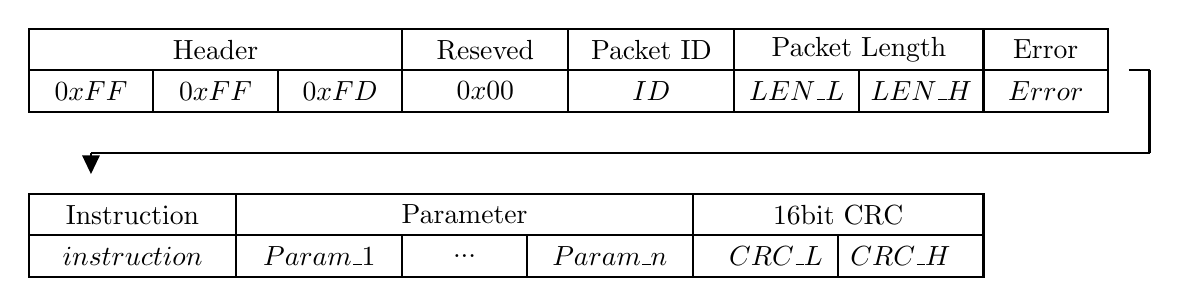
\begin{tikzpicture}[x=0.75pt,y=0.75pt,yscale=-1,xscale=1]
%uncomment if require: \path (0,158.99999237060547); %set diagram left start at 0, and has height of 158.99999237060547

%Shape: Rectangle [id:dp8698497909833363] 
\draw   (10,30) -- (70,30) -- (70,50) -- (10,50) -- cycle ;
%Shape: Rectangle [id:dp6485581117247297] 
\draw   (70,30) -- (130,30) -- (130,50) -- (70,50) -- cycle ;
%Shape: Rectangle [id:dp6658546174120246] 
\draw   (130,30) -- (190,30) -- (190,50) -- (130,50) -- cycle ;
%Shape: Rectangle [id:dp6752872057996913] 
\draw   (190,30) -- (270,30) -- (270,50) -- (190,50) -- cycle ;
%Shape: Rectangle [id:dp5014813538264575] 
\draw   (350,30) -- (410,30) -- (410,50) -- (350,50) -- cycle ;
%Shape: Rectangle [id:dp7457170593383808] 
\draw   (410,30) -- (470,30) -- (470,50) -- (410,50) -- cycle ;
%Shape: Rectangle [id:dp5054173748421811] 
\draw   (270,30) -- (350,30) -- (350,50) -- (270,50) -- cycle ;
%Shape: Rectangle [id:dp1263298518018401] 
\draw   (10,109.5) -- (110,109.5) -- (110,129.5) -- (10,129.5) -- cycle ;
%Shape: Rectangle [id:dp6896214683381987] 
\draw   (110,109.5) -- (190,109.5) -- (190,129.5) -- (110,129.5) -- cycle ;
%Shape: Rectangle [id:dp8350012688131694] 
\draw   (330,89.5) -- (470,89.5) -- (470,109.5) -- (330,109.5) -- cycle ;
%Shape: Rectangle [id:dp8375426281198146] 
\draw   (190,109.5) -- (250,109.5) -- (250,129.5) -- (190,129.5) -- cycle ;
%Shape: Rectangle [id:dp6586789788358929] 
\draw   (330,109.5) -- (400,109.5) -- (400,129.5) -- (330,129.5) -- cycle ;
%Shape: Rectangle [id:dp14973963332658702] 
\draw   (10,10) -- (190,10) -- (190,30) -- (10,30) -- cycle ;
%Shape: Rectangle [id:dp30939097077443956] 
\draw   (190,10) -- (270,10) -- (270,30) -- (190,30) -- cycle ;
%Shape: Rectangle [id:dp20452238276938295] 
\draw   (350,10) -- (470,10) -- (470,30) -- (350,30) -- cycle ;
%Shape: Rectangle [id:dp08631851455147288] 
\draw   (270,10) -- (350,10) -- (350,30) -- (270,30) -- cycle ;
%Shape: Rectangle [id:dp351731230245929] 
\draw   (10,89.5) -- (110,89.5) -- (110,109.5) -- (10,109.5) -- cycle ;
%Shape: Rectangle [id:dp46139057893485447] 
\draw   (250,109.5) -- (330,109.5) -- (330,129.5) -- (250,129.5) -- cycle ;
%Shape: Rectangle [id:dp42456037527605517] 
\draw   (110,89.5) -- (330,89.5) -- (330,109.5) -- (110,109.5) -- cycle ;
%Shape: Rectangle [id:dp5173327089860826] 
\draw   (400,109.5) -- (470,109.5) -- (470,129.5) -- (400,129.5) -- cycle ;
%Straight Lines [id:da19477344689590792] 
\draw    (550,70) -- (40,70) ;


%Straight Lines [id:da31415506805713345] 
\draw    (40,70) -- (40,78) ;
\draw [shift={(40,80)}, rotate = 270] [fill={rgb, 255:red, 0; green, 0; blue, 0 }  ][line width=0.75]  [draw opacity=0] (8.93,-4.29) -- (0,0) -- (8.93,4.29) -- cycle    ;

%Shape: Rectangle [id:dp13994941859002452] 
\draw   (470,10) -- (530,10) -- (530,30) -- (470,30) -- cycle ;
%Shape: Rectangle [id:dp04644653628071138] 
\draw   (470,30) -- (530,30) -- (530,50) -- (470,50) -- cycle ;
%Straight Lines [id:da3764266198993005] 
\draw    (550,70) -- (550,30) ;


%Straight Lines [id:da06827427289797416] 
\draw    (540,30) -- (550,30) ;



% Text Node
\draw (40,40) node   {$0xFF$};
% Text Node
\draw (100,40) node   {$0xFF$};
% Text Node
\draw (160,40) node   {$0xFD$};
% Text Node
\draw (100,20) node  [align=left] {Header};
% Text Node
\draw (230,20) node  [align=left] {Reseved};
% Text Node
\draw (230,40) node   {$0x00$};
% Text Node
\draw (310,40) node   {$ID$};
% Text Node
\draw (310,20) node  [align=left] {Packet ID};
% Text Node
\draw (380,40) node   {$LEN\_L$};
% Text Node
\draw (440,40) node   {$LEN\_H$};
% Text Node
\draw (410,20) node  [align=left] {Packet Length};
% Text Node
\draw (60,119.5) node   {$instruction$};
% Text Node
\draw (60,100) node  [align=left] {Instruction};
% Text Node
\draw (150,119.5) node   {$Param\_1$};
% Text Node
\draw (220,119.5) node   {$...$};
% Text Node
\draw (290,119.5) node   {$Param\_n$};
% Text Node
\draw (220,99.5) node  [align=left] {Parameter};
% Text Node
\draw (370,119.5) node   {$CRC\_L$};
% Text Node
\draw (430,119.5) node   {$CRC\_H$};
% Text Node
\draw (400,99.5) node  [align=left] {16bit CRC};
% Text Node
\draw (500,20) node  [align=left] {Error};
% Text Node
\draw (500,40) node   {$Error$};


\end{tikzpicture}

    \caption{Structure of the status packet}
    \label{fig:StatusStruct}
\end{figure}
As you can see from the only difference from the structure of the instruction packet is the error field.
This error field indicates the result of the instruction packet. The error field can be seen in the figure above. 
\begin{figure}[H]
    \centering
    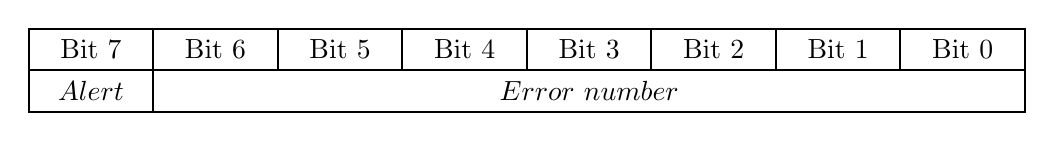
\begin{tikzpicture}[x=0.75pt,y=0.75pt,yscale=-1,xscale=1]
%uncomment if require: \path (0,158.99999237060547); %set diagram left start at 0, and has height of 158.99999237060547

%Shape: Rectangle [id:dp09142087079107619] 
\draw   (10,10) -- (70,10) -- (70,30) -- (10,30) -- cycle ;
%Shape: Rectangle [id:dp4629750443029259] 
\draw   (70,10) -- (130,10) -- (130,30) -- (70,30) -- cycle ;
%Shape: Rectangle [id:dp16194932941841267] 
\draw   (130,10) -- (190,10) -- (190,30) -- (130,30) -- cycle ;
%Shape: Rectangle [id:dp25658747620974176] 
\draw   (190,10) -- (250,10) -- (250,30) -- (190,30) -- cycle ;
%Shape: Rectangle [id:dp4454573381940983] 
\draw   (250,10) -- (310,10) -- (310,30) -- (250,30) -- cycle ;
%Shape: Rectangle [id:dp2107426327299584] 
\draw   (310,10) -- (370,10) -- (370,30) -- (310,30) -- cycle ;
%Shape: Rectangle [id:dp742699471984243] 
\draw   (370,10) -- (430,10) -- (430,30) -- (370,30) -- cycle ;
%Shape: Rectangle [id:dp768648200139064] 
\draw   (430,10) -- (490,10) -- (490,30) -- (430,30) -- cycle ;
%Shape: Rectangle [id:dp3416120520607919] 
\draw   (10,30) -- (70,30) -- (70,50) -- (10,50) -- cycle ;
%Shape: Rectangle [id:dp9451706315688295] 
\draw   (70,30) -- (490,30) -- (490,50) -- (70,50) -- cycle ;

% Text Node
\draw (40,20) node  [align=left] {Bit 7};
% Text Node
\draw (100,20) node  [align=left] {Bit 6};
% Text Node
\draw (160,20) node  [align=left] {Bit 5};
% Text Node
\draw (220,20) node  [align=left] {Bit 4};
% Text Node
\draw (280,20) node  [align=left] {Bit 3};
% Text Node
\draw (340,20) node  [align=left] {Bit 2};
% Text Node
\draw (400,20) node  [align=left] {Bit 1};
% Text Node
\draw (460,20) node  [align=left] {Bit 0};
% Text Node
\draw (40,40) node   {$Alert$};
% Text Node
\draw (280,40) node   {$Error\ number$};


\end{tikzpicture}

    \caption{Error structure\cite{PIDmxx}}
    \label{fig:Errorstruct}
\end{figure}
In bit number 7, the alert changes the value from 0 to 1 if there is a failure on the device. 
\begin{table}[H]
    \centering
    \begin{tabular}{|P{1.5cm}||P{2cm}||P{9cm}|}\hline
       \textbf{Value}  & \textbf{Error} & \textbf{Description} \\ \hline
        $0x01$ & Result fail &  failed to process the sent Instruction Packet\\ \hline
        $0x02$ & Instruction Error &  undefined Instruction has been used OR Action has been used without Reg Write\\ \hline
        $0x03$ & CRC Error &  CRC of the sent Packet does not match\\ \hline
        $0x04$ & Data range Error &  Data to be written in the corresponding Address is outside the range of the minimum/maximum value\\ \hline
        $0x05$ & Data Length Error &  Attempt to write Data that is shorter than the data length of the corresponding Address\\ \hline
        $0x06$ & Data Limit Error &  Data to be written in the corresponding Address is outside of the Limit value\\ \hline
        
        $0x07$ & 
        Access Error&  Attempt to write a value in an Address that is Read Only or has not been defined OR  attempt to read a value in an Address that is Write Only or has not been defined OR attempt to write a value in the ROM domain while in a state of Torque Enable(ROM Lock)\\ \hline
    \end{tabular}
    \caption{Table of errors on the status packet}
    \label{tab:Status Errors}
\end{table}


\paragraph{The Teensy microcontroller} is used as a data bridge between the MCP and the Dynamixel servos.
\subsection{CrustCrawler}
The robotic manipulator used in this project is a CrustCrawler arm consisting of one Dynamixel MX 106 SERVO, two Dynamixel MX 64 SERVO and two MX 28 Servos in the following setup:
\missingfigure{Picture of robot}

\section{Control Systems}
%Intro:
\begin{figure}[H]
    \centering
    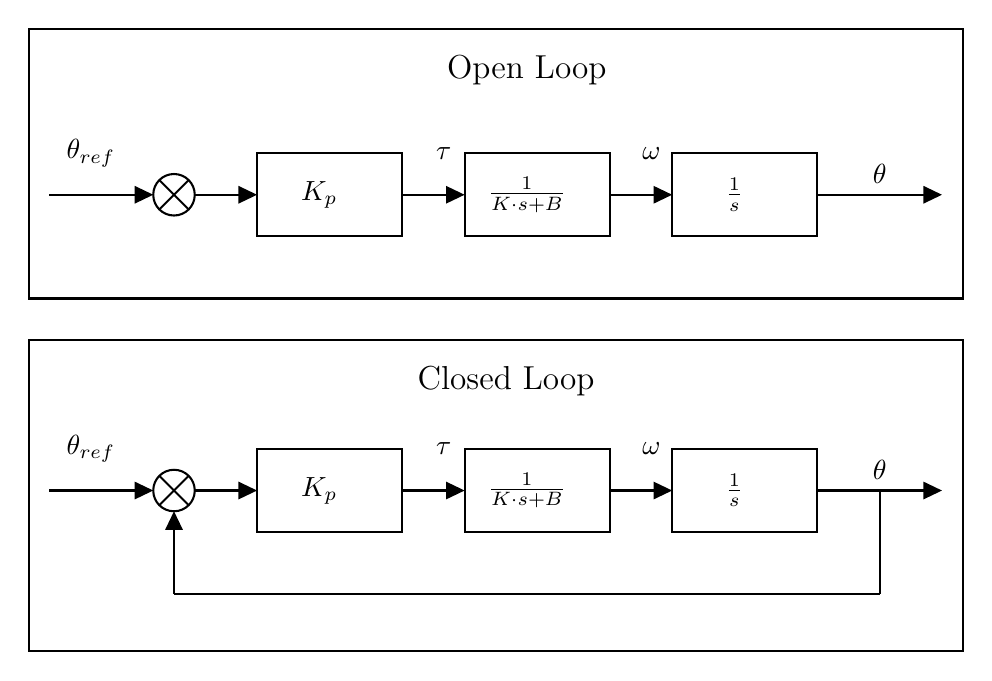
\begin{tikzpicture}[x=0.75pt,y=0.75pt,yscale=-1,xscale=1]
%uncomment if require: \path (0,328.50892877578735); %set diagram left start at 0, and has height of 328.50892877578735

%Shape: Rectangle [id:dp12482796861282974] 
\draw   (140,80) -- (210,80) -- (210,120) -- (140,120) -- cycle ;
%Straight Lines [id:da5706724332227189] 
\draw    (40,100) -- (88,100) ;
\draw [shift={(90,100)}, rotate = 180] [fill={rgb, 255:red, 0; green, 0; blue, 0 }  ][line width=0.75]  [draw opacity=0] (8.93,-4.29) -- (0,0) -- (8.93,4.29) -- cycle    ;

%Flowchart: Summing Junction [id:dp53704430353601] 
\draw   (90,100) .. controls (90,94.48) and (94.48,90) .. (100,90) .. controls (105.52,90) and (110,94.48) .. (110,100) .. controls (110,105.52) and (105.52,110) .. (100,110) .. controls (94.48,110) and (90,105.52) .. (90,100) -- cycle ; \draw   (92.93,92.93) -- (107.07,107.07) ; \draw   (107.07,92.93) -- (92.93,107.07) ;
%Straight Lines [id:da3178828171562029] 
\draw    (110,100) -- (138,100) ;
\draw [shift={(140,100)}, rotate = 180] [fill={rgb, 255:red, 0; green, 0; blue, 0 }  ][line width=0.75]  [draw opacity=0] (8.93,-4.29) -- (0,0) -- (8.93,4.29) -- cycle    ;

%Shape: Rectangle [id:dp28027349651381117] 
\draw   (240,80) -- (310,80) -- (310,120) -- (240,120) -- cycle ;
%Straight Lines [id:da11899224305491352] 
\draw    (210,100) -- (238,100) ;
\draw [shift={(240,100)}, rotate = 180] [fill={rgb, 255:red, 0; green, 0; blue, 0 }  ][line width=0.75]  [draw opacity=0] (8.93,-4.29) -- (0,0) -- (8.93,4.29) -- cycle    ;

%Shape: Rectangle [id:dp31656367205122615] 
\draw   (340,80) -- (410,80) -- (410,120) -- (340,120) -- cycle ;
%Straight Lines [id:da5367106543687827] 
\draw    (310,100) -- (338,100) ;
\draw [shift={(340,100)}, rotate = 180] [fill={rgb, 255:red, 0; green, 0; blue, 0 }  ][line width=0.75]  [draw opacity=0] (8.93,-4.29) -- (0,0) -- (8.93,4.29) -- cycle    ;

%Straight Lines [id:da7913281226659683] 
\draw    (410,100) -- (468,100) ;
\draw [shift={(470,100)}, rotate = 180] [fill={rgb, 255:red, 0; green, 0; blue, 0 }  ][line width=0.75]  [draw opacity=0] (8.93,-4.29) -- (0,0) -- (8.93,4.29) -- cycle    ;

%Shape: Rectangle [id:dp11142722632197088] 
\draw   (30,20) -- (480,20) -- (480,150) -- (30,150) -- cycle ;
%Shape: Rectangle [id:dp14600397799019293] 
\draw   (140,222.5) -- (210,222.5) -- (210,262.5) -- (140,262.5) -- cycle ;
%Straight Lines [id:da4243355948071521] 
\draw    (40,242.5) -- (88,242.5) ;
\draw [shift={(90,242.5)}, rotate = 180] [fill={rgb, 255:red, 0; green, 0; blue, 0 }  ][line width=0.75]  [draw opacity=0] (8.93,-4.29) -- (0,0) -- (8.93,4.29) -- cycle    ;

%Flowchart: Summing Junction [id:dp6729381602093008] 
\draw   (90,242.5) .. controls (90,236.98) and (94.48,232.5) .. (100,232.5) .. controls (105.52,232.5) and (110,236.98) .. (110,242.5) .. controls (110,248.02) and (105.52,252.5) .. (100,252.5) .. controls (94.48,252.5) and (90,248.02) .. (90,242.5) -- cycle ; \draw   (92.93,235.43) -- (107.07,249.57) ; \draw   (107.07,235.43) -- (92.93,249.57) ;
%Straight Lines [id:da14869215035902505] 
\draw    (110,242.5) -- (138,242.5) ;
\draw [shift={(140,242.5)}, rotate = 180] [fill={rgb, 255:red, 0; green, 0; blue, 0 }  ][line width=0.75]  [draw opacity=0] (8.93,-4.29) -- (0,0) -- (8.93,4.29) -- cycle    ;

%Shape: Rectangle [id:dp9900763090446374] 
\draw   (240,222.5) -- (310,222.5) -- (310,262.5) -- (240,262.5) -- cycle ;
%Straight Lines [id:da7760938350165698] 
\draw    (210,242.5) -- (238,242.5) ;
\draw [shift={(240,242.5)}, rotate = 180] [fill={rgb, 255:red, 0; green, 0; blue, 0 }  ][line width=0.75]  [draw opacity=0] (8.93,-4.29) -- (0,0) -- (8.93,4.29) -- cycle    ;

%Shape: Rectangle [id:dp19026495853512104] 
\draw   (340,222.5) -- (410,222.5) -- (410,262.5) -- (340,262.5) -- cycle ;
%Straight Lines [id:da42905616589605233] 
\draw    (310,242.5) -- (338,242.5) ;
\draw [shift={(340,242.5)}, rotate = 180] [fill={rgb, 255:red, 0; green, 0; blue, 0 }  ][line width=0.75]  [draw opacity=0] (8.93,-4.29) -- (0,0) -- (8.93,4.29) -- cycle    ;

%Straight Lines [id:da668486289799261] 
\draw    (410,242.5) -- (468,242.5) ;
\draw [shift={(470,242.5)}, rotate = 180] [fill={rgb, 255:red, 0; green, 0; blue, 0 }  ][line width=0.75]  [draw opacity=0] (8.93,-4.29) -- (0,0) -- (8.93,4.29) -- cycle    ;

%Straight Lines [id:da5740200387655516] 
\draw    (100,254.5) -- (100,292.5) ;

\draw [shift={(100,252.5)}, rotate = 90] [fill={rgb, 255:red, 0; green, 0; blue, 0 }  ][line width=0.75]  [draw opacity=0] (8.93,-4.29) -- (0,0) -- (8.93,4.29) -- cycle    ;
%Straight Lines [id:da1492709801617349] 
\draw    (100,292.5) -- (440,292.5) ;


%Straight Lines [id:da5671703763154259] 
\draw    (440,242.5) -- (440,292.5) ;


%Shape: Rectangle [id:dp043811444149466805] 
\draw   (30,170) -- (480,170) -- (480,320) -- (30,320) -- cycle ;

% Text Node
\draw (60,80) node   {$\theta _{ref}$};
% Text Node
\draw (170,100) node   {$K_{p}$};
% Text Node
\draw (230,80) node   {$\tau $};
% Text Node
\draw (270,100) node   {$\frac{1}{K\cdot s+B}$};
% Text Node
\draw (370,100) node   {$\frac{1}{s}$};
% Text Node
\draw (330,80) node   {$\omega $};
% Text Node
\draw (440,90) node   {$\theta $};
% Text Node
\draw (270,40) node  [align=left] {{\large Open Loop}};
% Text Node
\draw (60,222.5) node   {$\theta _{ref}$};
% Text Node
\draw (170,242.5) node   {$K_{p}$};
% Text Node
\draw (230,222.5) node   {$\tau $};
% Text Node
\draw (270,242.5) node   {$\frac{1}{K\cdot s+B}$};
% Text Node
\draw (370,242.5) node   {$\frac{1}{s}$};
% Text Node
\draw (330,222.5) node   {$\omega $};
% Text Node
\draw (440,232.5) node   {$\theta $};
% Text Node
\draw (260,190) node  [align=left] {{\large Closed Loop}};


\end{tikzpicture}

    \caption{Open- and closed loop are control schemes and that show how the signal runs through a controller}
    \label{fig:openclose}
\end{figure}
As seen on the figure \ref{fig:openclose}, open loop, it manages to compute the reference signal and regulate it so that it is equal to the desired output. If a  disturbance were introduced to the open loop system, the system could not adjust for the disturbance and would produce an unrecognisable error.\\
In the closed-loop system/feedback loop we can measure the output error and measure it towards the input and try to eliminate the error of disturbances to make the system linear, and easier to work with, but this is another section that will be covered in \ref{PID}.\\ 
Utilising these control systems can be done by transfer functions. Transfer functions is the Laplace formulae of the control system design.\\

\subsection{The Golden Formula}
\begin{figure}[H]
    \centering
    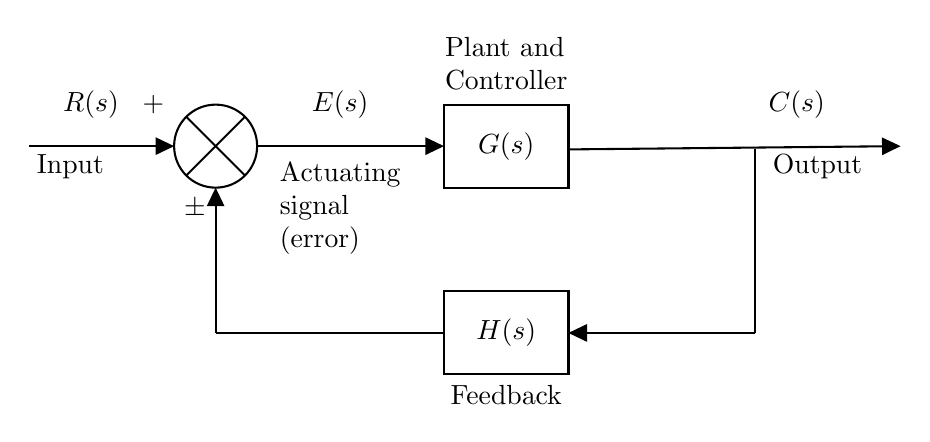
\begin{tikzpicture}[x=0.75pt,y=0.75pt,yscale=-1,xscale=1]
%uncomment if require: \path (0,300); %set diagram left start at 0, and has height of 300

%Straight Lines
\draw    (10,68.71) -- (78,68.71) ;
\draw [shift={(80,68.71)}, rotate = 180] [fill={rgb, 255:red, 0; green, 0; blue, 0 }  ][line width=0.75]  [draw opacity=0] (8.93,-4.29) -- (0,0) -- (8.93,4.29) -- cycle    ;

%Flowchart: Summing Junction
\draw   (80,68.71) .. controls (80,57.67) and (88.95,48.71) .. (100,48.71) .. controls (111.05,48.71) and (120,57.67) .. (120,68.71) .. controls (120,79.76) and (111.05,88.71) .. (100,88.71) .. controls (88.95,88.71) and (80,79.76) .. (80,68.71) -- cycle ; \draw   (85.86,54.57) -- (114.14,82.86) ; \draw   (114.14,54.57) -- (85.86,82.86) ;
%Straight Lines
\draw    (120,68.71) -- (208,68.71) ;
\draw [shift={(210,68.71)}, rotate = 180] [fill={rgb, 255:red, 0; green, 0; blue, 0 }  ][line width=0.75]  [draw opacity=0] (8.93,-4.29) -- (0,0) -- (8.93,4.29) -- cycle    ;

%Shape: Rectangle
\draw   (210,48.71) -- (270,48.71) -- (270,88.71) -- (210,88.71) -- cycle ;
%Straight Lines
\draw    (270,70.29) -- (428,68.73) ;
\draw [shift={(430,68.71)}, rotate = 539.44] [fill={rgb, 255:red, 0; green, 0; blue, 0 }  ][line width=0.75]  [draw opacity=0] (8.93,-4.29) -- (0,0) -- (8.93,4.29) -- cycle    ;

%Straight Lines
\draw    (360,70.29) -- (360,158.71) ;


%Straight Lines
\draw    (360,158.71) -- (272,158.71) ;
\draw [shift={(270,158.71)}, rotate = 360] [fill={rgb, 255:red, 0; green, 0; blue, 0 }  ][line width=0.75]  [draw opacity=0] (8.93,-4.29) -- (0,0) -- (8.93,4.29) -- cycle    ;

%Shape: Rectangle
\draw   (210,138.71) -- (270,138.71) -- (270,178.71) -- (210,178.71) -- cycle ;
%Straight Lines
\draw    (210,158.71) -- (100,158.71) ;


%Straight Lines
\draw    (100,158.71) -- (100,90.71) ;
\draw [shift={(100,88.71)}, rotate = 450] [fill={rgb, 255:red, 0; green, 0; blue, 0 }  ][line width=0.75]  [draw opacity=0] (8.93,-4.29) -- (0,0) -- (8.93,4.29) -- cycle    ;


% Text Node
\draw (40,48.71) node   {$R( s)$};
% Text Node
\draw (70,48.71) node   {$+$};
% Text Node
\draw (160,48.71) node   {$E( s)$};
% Text Node
\draw (240,68.71) node   {$G( s)$};
% Text Node
\draw (380,48.71) node   {$C( s)$};
% Text Node
\draw (240,158.71) node   {$H( s)$};
% Text Node
\draw (90,98.71) node   {$\pm $};
% Text Node
\draw (160,98.71) node  [align=left] {Actuating \\signal\\(error)};
% Text Node
\draw (30,78.71) node  [align=left] {Input};
% Text Node
\draw (390,78.71) node  [align=left] {Output};
% Text Node
\draw (240,188.71) node  [align=left] {Feedback};
% Text Node
\draw (240,28.71) node  [align=left] {Plant and \\Controller};


\end{tikzpicture}
    \caption{Standard format feedback loop here Arrows signify signals and boxes mechanisms, this standard form feedback loop are used to illustrate the golden formula}
    \label{fig:FeedbackLoop}
\end{figure}
When working with the standard setup of a feedback loop the use of the Golden Formula can describe the output $C(s)$ depending on the input $R(s)$.
\begin{equation}\label{eq:GoldenFormula}
    C(s)=\frac{G(s)}{1\mp G(s)\cdot H(s)}\cdot R(s)
\end{equation}
The transfer function given by the Golden Formula, this is what is called the closed-loop transfer function, the product $G(s)\cdot H(s)$ is called the open-loop transfer-function, or loop-gain.



\subsection{Signal analysis}
When working with sinusoidal signals there are terms to describe the signal. Figure \ref{fig:StepRespGraf} illustrates some of these terms graphically on a step response signal.

\begin{figure}[H]
 \centering 
    \includegraphics[scale=0.8]{Figures/StepResponse1.jpg}
    \caption{Figure with using step response signal, terms marked graphically in figure\cite{Risetime76:online}.}
    \label{fig:StepRespGraf}
\end{figure}

\begin{itemize}
    \item \textbf{Rise time} refers to the duration it takes for the step response y(t) from 10\% to 90\% of the final steady-state of the response\cite{Risetime76:online}.
    
    \item \textbf{Settling time} is the time it takes for y(t) reach and stay within the steady state, which is  +/- 2\% of $y_{final}$ (the steady state value)\cite{Risetime76:online}.
   
    \item \textbf{Percent overshoot} is the overshoot y(t) reaches relative to the steady state value $y_{final}$\cite{Risetime76:online}.

    \item \textbf{Peak} is highest value y(t) reaches\cite{Risetime76:online}.

    \item \textbf{Peak time} is the time it takes  for y(t) reach its first/maximum value\cite{Risetime76:online}. 
    
\end{itemize}
\newpage
\subsection{Controller design} \label{PID}
There are one specific controller that is related to this project, the PID (Proportional, Integral, Derivative) controller. This PID controller is used to delimit the errors inside a loop. Each of these Components driving the error to zero, which can be read about in the sections to come. Every component has its own allocated gain, a gain is the ratio between the output divide by the input. The objective in this system is to move from one angle to another, the error would then be difference in angles over time. In this section \textbf{\textit{U}} is denoted as being the effort to be put in the system.\\

\begin{figure}
    \centering
    

\tikzset{every picture/.style={line width=0.75pt}} %set default line width to 0.75pt        

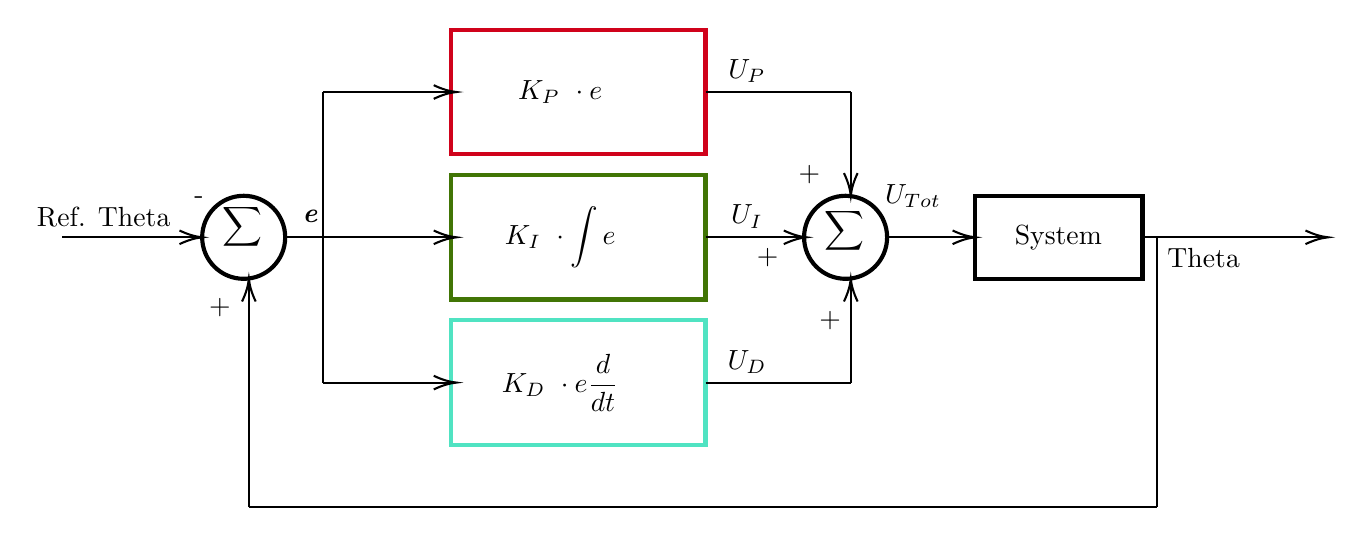
\begin{tikzpicture}[x=0.75pt,y=0.75pt,yscale=-1,xscale=1]
%uncomment if require: \path (0,269); %set diagram left start at 0, and has height of 269

%Shape: Rectangle [id:dp6186698400269734] 
\draw  [color={rgb, 255:red, 208; green, 2; blue, 27 }  ,draw opacity=1 ][line width=1.5]  (217.5,20) -- (340,20) -- (340,80) -- (217.5,80) -- cycle ;
%Shape: Rectangle [id:dp35497397654468] 
\draw  [color={rgb, 255:red, 65; green, 117; blue, 5 }  ,draw opacity=1 ][line width=1.5]  (217.5,90) -- (340,90) -- (340,150) -- (217.5,150) -- cycle ;
%Shape: Rectangle [id:dp0011241398633399236] 
\draw  [color={rgb, 255:red, 80; green, 227; blue, 194 }  ,draw opacity=1 ][line width=1.5]  (217.5,160) -- (340,160) -- (340,220) -- (217.5,220) -- cycle ;
%Shape: Circle [id:dp7081049529214984] 
\draw  [line width=1.5]  (97.5,120) .. controls (97.5,108.95) and (106.45,100) .. (117.5,100) .. controls (128.55,100) and (137.5,108.95) .. (137.5,120) .. controls (137.5,131.05) and (128.55,140) .. (117.5,140) .. controls (106.45,140) and (97.5,131.05) .. (97.5,120) -- cycle ;
%Straight Lines [id:da1012548517194285] 
\draw    (155.61,50) -- (218,50) ;
\draw [shift={(220,50)}, rotate = 180] [color={rgb, 255:red, 0; green, 0; blue, 0 }  ][line width=0.75]    (10.93,-3.29) .. controls (6.95,-1.4) and (3.31,-0.3) .. (0,0) .. controls (3.31,0.3) and (6.95,1.4) .. (10.93,3.29)   ;

%Straight Lines [id:da024552935574742696] 
\draw    (137.5,120) -- (218,120) ;
\draw [shift={(220,120)}, rotate = 180] [color={rgb, 255:red, 0; green, 0; blue, 0 }  ][line width=0.75]    (10.93,-3.29) .. controls (6.95,-1.4) and (3.31,-0.3) .. (0,0) .. controls (3.31,0.3) and (6.95,1.4) .. (10.93,3.29)   ;

%Straight Lines [id:da632489535879416] 
\draw    (155.61,190) -- (218,190) ;
\draw [shift={(220,190)}, rotate = 180] [color={rgb, 255:red, 0; green, 0; blue, 0 }  ][line width=0.75]    (10.93,-3.29) .. controls (6.95,-1.4) and (3.31,-0.3) .. (0,0) .. controls (3.31,0.3) and (6.95,1.4) .. (10.93,3.29)   ;

%Straight Lines [id:da028164362822356237] 
\draw    (155.61,50) -- (155.61,110) ;


%Straight Lines [id:da1783990189247291] 
\draw    (155.61,110) -- (155.61,190) ;


%Shape: Ellipse [id:dp13776991374733094] 
\draw  [line width=1.5]  (387.5,120) .. controls (387.5,108.95) and (396.45,100) .. (407.5,100) .. controls (418.55,100) and (427.5,108.95) .. (427.5,120) .. controls (427.5,131.05) and (418.55,140) .. (407.5,140) .. controls (396.45,140) and (387.5,131.05) .. (387.5,120) -- cycle ;
%Straight Lines [id:da5590648239872058] 
\draw    (340,50) -- (410,50) ;


%Straight Lines [id:da32339100567036794] 
\draw    (340,120) -- (386.65,120) ;
\draw [shift={(388.65,120)}, rotate = 180] [color={rgb, 255:red, 0; green, 0; blue, 0 }  ][line width=0.75]    (10.93,-3.29) .. controls (6.95,-1.4) and (3.31,-0.3) .. (0,0) .. controls (3.31,0.3) and (6.95,1.4) .. (10.93,3.29)   ;

%Straight Lines [id:da37714274354973676] 
\draw    (340,190) -- (410,190) ;


%Straight Lines [id:da12414839144602552] 
\draw    (410,50) -- (410,98) ;
\draw [shift={(410,100)}, rotate = 270] [color={rgb, 255:red, 0; green, 0; blue, 0 }  ][line width=0.75]    (10.93,-3.29) .. controls (6.95,-1.4) and (3.31,-0.3) .. (0,0) .. controls (3.31,0.3) and (6.95,1.4) .. (10.93,3.29)   ;

%Straight Lines [id:da2294854556231043] 
\draw    (410,142) -- (410,190) ;

\draw [shift={(410,140)}, rotate = 90] [color={rgb, 255:red, 0; green, 0; blue, 0 }  ][line width=0.75]    (10.93,-3.29) .. controls (6.95,-1.4) and (3.31,-0.3) .. (0,0) .. controls (3.31,0.3) and (6.95,1.4) .. (10.93,3.29)   ;
%Straight Lines [id:da7636925489142845] 
\draw    (427.5,120) -- (468,120) ;
\draw [shift={(470,120)}, rotate = 180] [color={rgb, 255:red, 0; green, 0; blue, 0 }  ][line width=0.75]    (10.93,-3.29) .. controls (6.95,-1.4) and (3.31,-0.3) .. (0,0) .. controls (3.31,0.3) and (6.95,1.4) .. (10.93,3.29)   ;

%Straight Lines [id:da8120471221631163] 
\draw    (30,120) -- (95.5,120) ;
\draw [shift={(97.5,120)}, rotate = 180] [color={rgb, 255:red, 0; green, 0; blue, 0 }  ][line width=0.75]    (10.93,-3.29) .. controls (6.95,-1.4) and (3.31,-0.3) .. (0,0) .. controls (3.31,0.3) and (6.95,1.4) .. (10.93,3.29)   ;

%Straight Lines [id:da7263862005723072] 
\draw    (120,250) -- (120,142) ;
\draw [shift={(120,140)}, rotate = 450] [color={rgb, 255:red, 0; green, 0; blue, 0 }  ][line width=0.75]    (10.93,-3.29) .. controls (6.95,-1.4) and (3.31,-0.3) .. (0,0) .. controls (3.31,0.3) and (6.95,1.4) .. (10.93,3.29)   ;

%Straight Lines [id:da9777886662003494] 
\draw    (120,250) -- (490,250) ;


%Shape: Rectangle [id:dp7284343716119925] 
\draw  [line width=1.5]  (470,100) -- (550.53,100) -- (550.53,140) -- (470,140) -- cycle ;
%Straight Lines [id:da4771680795774551] 
\draw    (550.53,120) -- (638,120) ;
\draw [shift={(640,120)}, rotate = 180] [color={rgb, 255:red, 0; green, 0; blue, 0 }  ][line width=0.75]    (10.93,-3.29) .. controls (6.95,-1.4) and (3.31,-0.3) .. (0,0) .. controls (3.31,0.3) and (6.95,1.4) .. (10.93,3.29)   ;

%Straight Lines [id:da7739849283065594] 
\draw    (557.37,120) -- (557.37,250) ;


%Straight Lines [id:da5629774692956326] 
\draw    (557.37,250) -- (485.79,250) ;



% Text Node
\draw (50,110) node  [align=left] {Ref. Theta};
% Text Node
\draw (510,120) node  [align=left] {System};
% Text Node
\draw (270,190) node  [align=left] {$\displaystyle K_{D} \ \cdot e  \frac{d}{dt}$};
% Text Node
\draw (270,120) node  [align=left] {$\displaystyle K_{I} \ \cdot \int e$};
% Text Node
\draw (270,50) node  [align=left] {$\displaystyle K_{P} \ \cdot e$};
% Text Node
\draw (390,90) node  [align=left] {+};
% Text Node
\draw (370,130) node  [align=left] {+};
% Text Node
\draw (400,160) node  [align=left] {+};
% Text Node
\draw (106,154) node  [align=left] {+};
% Text Node
\draw (96,101) node  [align=left] {\mbox{-}};
% Text Node
\draw (150,110) node  [align=left] {\textit{\textbf{e}}};
% Text Node
\draw (407,117) node  [align=left] {$\displaystyle \sum $};
% Text Node
\draw (360,110) node  [align=left] {$\displaystyle U_{I}$};
% Text Node
\draw (360,180) node  [align=left] {$\displaystyle U_{D}$};
% Text Node
\draw (360,40) node  [align=left] {$\displaystyle U_{P}$};
% Text Node
\draw (117,115) node  [align=left] {$\displaystyle \sum $};
% Text Node
\draw (440,100) node  [align=left] {$\displaystyle U_{Tot}$};
% Text Node
\draw (580,130) node  [align=left] {Theta};


\end{tikzpicture}

    %\includegraphics{Figures/Technical_figures/1-25.jpg}
    \caption{Layout of a PID controllers response on the error}
    \label{fig:mPID}
\end{figure}


\begin{equation}\label{PID}
    U=K_P\cdot\textit{e}+K_I\cdot\int\textit{e}+K_D\cdot\textit{e}\frac{d}{dt}
\end{equation}

\paragraph{The Proportional} gain $K_P$ in eq.\ref{PID} is the gain multiplied with the error(e) in eq. \ref{PID}, resulting in the effort. The larger gain a fast rise time, the rise time is the time it takes from 10\% to 90\% of the final angle. However this controller can only be used alone when the system can tolerate a constant error in steady state, a steady state error is an error over time that does not diminish. The proportional gain also has a tendency to overshoot the desired value if the gain is too high\cite{Control1DK}.\\

\begin{figure}[H]
    \centering
    \includegraphics[width=\textwidth]{Figures/Technical_figures/PGAIN.png} 
    %

\tikzset{every picture/.style={line width=0.75pt}} %set default line width to 0.75pt        

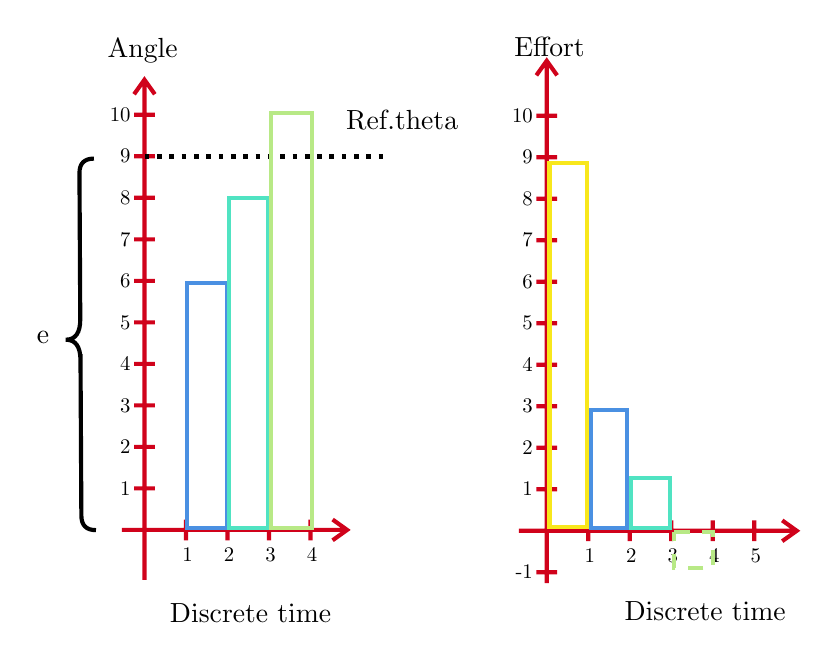
\begin{tikzpicture}[x=0.75pt,y=0.75pt,yscale=-1,xscale=1]
%uncomment if require: \path (0,530); %set diagram left start at 0, and has height of 530

%Shape: Axis 2D [id:dp45682595351826527] 
\draw [color={rgb, 255:red, 208; green, 2; blue, 27 }  ,draw opacity=1 ][line width=1.5]  (90,242.9) -- (198.5,242.9)(100.85,26) -- (100.85,267) (191.5,237.9) -- (198.5,242.9) -- (191.5,247.9) (95.85,33) -- (100.85,26) -- (105.85,33) (120.85,237.9) -- (120.85,247.9)(140.85,237.9) -- (140.85,247.9)(160.85,237.9) -- (160.85,247.9)(180.85,237.9) -- (180.85,247.9)(95.85,222.9) -- (105.85,222.9)(95.85,202.9) -- (105.85,202.9)(95.85,182.9) -- (105.85,182.9)(95.85,162.9) -- (105.85,162.9)(95.85,142.9) -- (105.85,142.9)(95.85,122.9) -- (105.85,122.9)(95.85,102.9) -- (105.85,102.9)(95.85,82.9) -- (105.85,82.9)(95.85,62.9) -- (105.85,62.9)(95.85,42.9) -- (105.85,42.9) ;
\draw   (127.85,254.9) node[anchor=east, scale=0.75]{1} (147.85,254.9) node[anchor=east, scale=0.75]{2} (167.85,254.9) node[anchor=east, scale=0.75]{3} (187.85,254.9) node[anchor=east, scale=0.75]{4} (97.85,222.9) node[anchor=east, scale=0.75]{1} (97.85,202.9) node[anchor=east, scale=0.75]{2} (97.85,182.9) node[anchor=east, scale=0.75]{3} (97.85,162.9) node[anchor=east, scale=0.75]{4} (97.85,142.9) node[anchor=east, scale=0.75]{5} (97.85,122.9) node[anchor=east, scale=0.75]{6} (97.85,102.9) node[anchor=east, scale=0.75]{7} (97.85,82.9) node[anchor=east, scale=0.75]{8} (97.85,62.9) node[anchor=east, scale=0.75]{9} (97.85,42.9) node[anchor=east, scale=0.75]{10} ;
%Straight Lines [id:da07124731425948538] 
\draw [line width=1.5]  [dash pattern={on 1.69pt off 2.76pt}]  (101,63) -- (218.5,63) ;


%Shape: Brace [id:dp5273011604952158] 
\draw  [line width=1.5]  (76.5,64) .. controls (71.83,64.03) and (69.51,66.37) .. (69.54,71.04) -- (69.93,141.23) .. controls (69.97,147.9) and (67.66,151.24) .. (62.99,151.27) .. controls (67.66,151.24) and (70.01,154.56) .. (70.04,161.23)(70.03,158.23) -- (70.46,236.04) .. controls (70.49,240.71) and (72.83,243.03) .. (77.5,243) ;
%Shape: Rectangle [id:dp5387283033097741] 
\draw  [color={rgb, 255:red, 74; green, 144; blue, 226 }  ,draw opacity=1 ][line width=1.5]  (121.5,124) -- (140.5,124) -- (140.5,242) -- (121.5,242) -- cycle ;
%Shape: Rectangle [id:dp6947960238766453] 
\draw  [color={rgb, 255:red, 80; green, 227; blue, 194 }  ,draw opacity=1 ][line width=1.5]  (141.67,83) -- (160.5,83) -- (160.5,242) -- (141.67,242) -- cycle ;
%Shape: Rectangle [id:dp8600292583953892] 
\draw  [color={rgb, 255:red, 184; green, 233; blue, 134 }  ,draw opacity=1 ][line width=1.5]  (161.67,42) -- (181.67,42) -- (181.67,242) -- (161.67,242) -- cycle ;
%Shape: Axis 2D [id:dp2561048365476184] 
\draw [color={rgb, 255:red, 208; green, 2; blue, 27 }  ,draw opacity=1 ][line width=1.5]  (281.28,243.33) -- (415.13,243.33)(294.67,16.89) -- (294.67,268.49) (408.13,238.33) -- (415.13,243.33) -- (408.13,248.33) (289.67,23.89) -- (294.67,16.89) -- (299.67,23.89) (314.67,238.33) -- (314.67,248.33)(334.67,238.33) -- (334.67,248.33)(354.67,238.33) -- (354.67,248.33)(374.67,238.33) -- (374.67,248.33)(394.67,238.33) -- (394.67,248.33)(289.67,223.33) -- (299.67,223.33)(289.67,203.33) -- (299.67,203.33)(289.67,183.33) -- (299.67,183.33)(289.67,163.33) -- (299.67,163.33)(289.67,143.33) -- (299.67,143.33)(289.67,123.33) -- (299.67,123.33)(289.67,103.33) -- (299.67,103.33)(289.67,83.33) -- (299.67,83.33)(289.67,63.33) -- (299.67,63.33)(289.67,43.33) -- (299.67,43.33)(289.67,263.33) -- (299.67,263.33) ;
\draw   (321.67,255.33) node[anchor=east, scale=0.75]{1} (341.67,255.33) node[anchor=east, scale=0.75]{2} (361.67,255.33) node[anchor=east, scale=0.75]{3} (381.67,255.33) node[anchor=east, scale=0.75]{4} (401.67,255.33) node[anchor=east, scale=0.75]{5} (291.67,223.33) node[anchor=east, scale=0.75]{1} (291.67,203.33) node[anchor=east, scale=0.75]{2} (291.67,183.33) node[anchor=east, scale=0.75]{3} (291.67,163.33) node[anchor=east, scale=0.75]{4} (291.67,143.33) node[anchor=east, scale=0.75]{5} (291.67,123.33) node[anchor=east, scale=0.75]{6} (291.67,103.33) node[anchor=east, scale=0.75]{7} (291.67,83.33) node[anchor=east, scale=0.75]{8} (291.67,63.33) node[anchor=east, scale=0.75]{9} (291.67,43.33) node[anchor=east, scale=0.75]{10} (291.67,263.33) node[anchor=east, scale=0.75]{-1} ;
%Shape: Rectangle [id:dp9341644709395209] 
\draw  [color={rgb, 255:red, 248; green, 231; blue, 28 }  ,draw opacity=1 ][line width=1.5]  (296,66) -- (314,66) -- (314,241.33) -- (296,241.33) -- cycle ;
%Shape: Rectangle [id:dp4499585049078272] 
\draw  [color={rgb, 255:red, 74; green, 144; blue, 226 }  ,draw opacity=1 ][line width=1.5]  (315.83,185) -- (333.33,185) -- (333.33,242) -- (315.83,242) -- cycle ;
%Shape: Rectangle [id:dp5245979736475872] 
\draw  [color={rgb, 255:red, 80; green, 227; blue, 194 }  ,draw opacity=1 ][line width=1.5]  (335.33,218) -- (354,218) -- (354,242) -- (335.33,242) -- cycle ;
%Shape: Rectangle [id:dp4864189057319952] 
\draw  [color={rgb, 255:red, 184; green, 233; blue, 134 }  ,draw opacity=1 ][dash pattern={on 5.63pt off 4.5pt}][line width=1.5]  (356,244) -- (374.67,244) -- (374.67,261.33) -- (356,261.33) -- cycle ;

% Text Node
\draw (225,45.33) node  [align=left] {Ref.theta};
% Text Node
\draw (52,150) node  [align=left] {e};
% Text Node
\draw (100,12) node  [align=left] {Angle};
% Text Node
\draw (152,283) node  [align=left] {Discrete time};
% Text Node
\draw (296,10) node  [align=left] {Effort};
% Text Node
\draw (371,282) node  [align=left] {Discrete time};


\end{tikzpicture}

    \caption{A $K_P$ of 1 then only the error has and effect on the effort}
    \label{fig:pGain}
\end{figure}

\paragraph{The Integral} gain $K_I$ in eq. \ref{PID} of the controller, accumulates error over time to output an effort to be put in the system. This means that it has a damping effect on the system. This Integral component can be used to minimise overshoot and eliminated the steady state error, that is in the p gain alone. This system accomplish this at the cost of a slow rise time. Thereby being slower to reach its desired destination than with a P gain alone, but will reach there in time. As safety is important when working with people this system would be very suited. However as this is a slow system the precision should be weighed against speed\cite{Control1DK}. \\

\begin{figure}[H]
    \centering
    \includegraphics[width=\textwidth]{Figures/Technical_figures/IGAIN.png} 
    %

\tikzset{every picture/.style={line width=0.75pt}} %set default line width to 0.75pt        

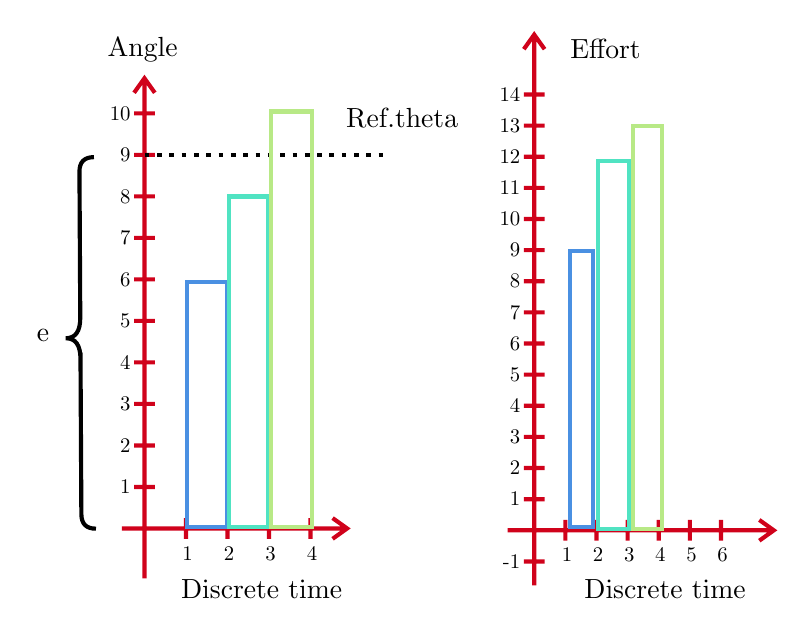
\begin{tikzpicture}[x=0.75pt,y=0.75pt,yscale=-1,xscale=1]
%uncomment if require: \path (0,530); %set diagram left start at 0, and has height of 530

%Shape: Axis 2D [id:dp6346571706526563] 
\draw [color={rgb, 255:red, 208; green, 2; blue, 27 }  ,draw opacity=1 ][line width=1.5]  (86,259.9) -- (194.5,259.9)(96.85,43) -- (96.85,284) (187.5,254.9) -- (194.5,259.9) -- (187.5,264.9) (91.85,50) -- (96.85,43) -- (101.85,50) (116.85,254.9) -- (116.85,264.9)(136.85,254.9) -- (136.85,264.9)(156.85,254.9) -- (156.85,264.9)(176.85,254.9) -- (176.85,264.9)(91.85,239.9) -- (101.85,239.9)(91.85,219.9) -- (101.85,219.9)(91.85,199.9) -- (101.85,199.9)(91.85,179.9) -- (101.85,179.9)(91.85,159.9) -- (101.85,159.9)(91.85,139.9) -- (101.85,139.9)(91.85,119.9) -- (101.85,119.9)(91.85,99.9) -- (101.85,99.9)(91.85,79.9) -- (101.85,79.9)(91.85,59.9) -- (101.85,59.9) ;
\draw   (123.85,271.9) node[anchor=east, scale=0.75]{1} (143.85,271.9) node[anchor=east, scale=0.75]{2} (163.85,271.9) node[anchor=east, scale=0.75]{3} (183.85,271.9) node[anchor=east, scale=0.75]{4} (93.85,239.9) node[anchor=east, scale=0.75]{1} (93.85,219.9) node[anchor=east, scale=0.75]{2} (93.85,199.9) node[anchor=east, scale=0.75]{3} (93.85,179.9) node[anchor=east, scale=0.75]{4} (93.85,159.9) node[anchor=east, scale=0.75]{5} (93.85,139.9) node[anchor=east, scale=0.75]{6} (93.85,119.9) node[anchor=east, scale=0.75]{7} (93.85,99.9) node[anchor=east, scale=0.75]{8} (93.85,79.9) node[anchor=east, scale=0.75]{9} (93.85,59.9) node[anchor=east, scale=0.75]{10} ;
%Straight Lines [id:da8395435041805068] 
\draw [line width=1.5]  [dash pattern={on 1.69pt off 2.76pt}]  (97,80) -- (214.5,80) ;


%Shape: Brace [id:dp15804314182279944] 
\draw  [line width=1.5]  (72.5,81) .. controls (67.83,81.03) and (65.51,83.37) .. (65.54,88.04) -- (65.93,158.23) .. controls (65.97,164.9) and (63.66,168.24) .. (58.99,168.27) .. controls (63.66,168.24) and (66.01,171.56) .. (66.04,178.23)(66.03,175.23) -- (66.46,253.04) .. controls (66.49,257.71) and (68.83,260.03) .. (73.5,260) ;
%Shape: Rectangle [id:dp5191693992255162] 
\draw  [color={rgb, 255:red, 74; green, 144; blue, 226 }  ,draw opacity=1 ][line width=1.5]  (117.5,141) -- (136.5,141) -- (136.5,259) -- (117.5,259) -- cycle ;
%Shape: Rectangle [id:dp2287664558829514] 
\draw  [color={rgb, 255:red, 80; green, 227; blue, 194 }  ,draw opacity=1 ][line width=1.5]  (137.67,100) -- (156.5,100) -- (156.5,259) -- (137.67,259) -- cycle ;
%Shape: Rectangle [id:dp3261576138135398] 
\draw  [color={rgb, 255:red, 184; green, 233; blue, 134 }  ,draw opacity=1 ][line width=1.5]  (157.67,59) -- (177.67,59) -- (177.67,259) -- (157.67,259) -- cycle ;
%Shape: Axis 2D [id:dp473563119637739] 
\draw [color={rgb, 255:red, 208; green, 2; blue, 27 }  ,draw opacity=1 ][line width=1.5]  (271.82,260.8) -- (400.08,260.8)(284.64,22) -- (284.64,287.33) (393.08,255.8) -- (400.08,260.8) -- (393.08,265.8) (279.64,29) -- (284.64,22) -- (289.64,29) (299.64,255.8) -- (299.64,265.8)(314.64,255.8) -- (314.64,265.8)(329.64,255.8) -- (329.64,265.8)(344.64,255.8) -- (344.64,265.8)(359.64,255.8) -- (359.64,265.8)(374.64,255.8) -- (374.64,265.8)(279.64,245.8) -- (289.64,245.8)(279.64,230.8) -- (289.64,230.8)(279.64,215.8) -- (289.64,215.8)(279.64,200.8) -- (289.64,200.8)(279.64,185.8) -- (289.64,185.8)(279.64,170.8) -- (289.64,170.8)(279.64,155.8) -- (289.64,155.8)(279.64,140.8) -- (289.64,140.8)(279.64,125.8) -- (289.64,125.8)(279.64,110.8) -- (289.64,110.8)(279.64,95.8) -- (289.64,95.8)(279.64,80.8) -- (289.64,80.8)(279.64,65.8) -- (289.64,65.8)(279.64,50.8) -- (289.64,50.8)(279.64,275.8) -- (289.64,275.8) ;
\draw   (306.64,272.8) node[anchor=east, scale=0.75]{1} (321.64,272.8) node[anchor=east, scale=0.75]{2} (336.64,272.8) node[anchor=east, scale=0.75]{3} (351.64,272.8) node[anchor=east, scale=0.75]{4} (366.64,272.8) node[anchor=east, scale=0.75]{5} (381.64,272.8) node[anchor=east, scale=0.75]{6} (281.64,245.8) node[anchor=east, scale=0.75]{1} (281.64,230.8) node[anchor=east, scale=0.75]{2} (281.64,215.8) node[anchor=east, scale=0.75]{3} (281.64,200.8) node[anchor=east, scale=0.75]{4} (281.64,185.8) node[anchor=east, scale=0.75]{5} (281.64,170.8) node[anchor=east, scale=0.75]{6} (281.64,155.8) node[anchor=east, scale=0.75]{7} (281.64,140.8) node[anchor=east, scale=0.75]{8} (281.64,125.8) node[anchor=east, scale=0.75]{9} (281.64,110.8) node[anchor=east, scale=0.75]{10} (281.64,95.8) node[anchor=east, scale=0.75]{11} (281.64,80.8) node[anchor=east, scale=0.75]{12} (281.64,65.8) node[anchor=east, scale=0.75]{13} (281.64,50.8) node[anchor=east, scale=0.75]{14} (281.64,275.8) node[anchor=east, scale=0.75]{-1} ;
%Shape: Rectangle [id:dp06820965849131166] 
\draw  [color={rgb, 255:red, 74; green, 144; blue, 226 }  ,draw opacity=1 ][line width=1.5]  (301.75,126.33) -- (313.08,126.33) -- (313.08,259) -- (301.75,259) -- cycle ;
%Shape: Rectangle [id:dp16997023555555235] 
\draw  [color={rgb, 255:red, 80; green, 227; blue, 194 }  ,draw opacity=1 ][line width=1.5]  (315.5,82.67) -- (330.5,82.67) -- (330.5,260) -- (315.5,260) -- cycle ;
%Shape: Rectangle [id:dp21980087841289575] 
\draw  [color={rgb, 255:red, 184; green, 233; blue, 134 }  ,draw opacity=1 ][line width=1.5]  (332.08,66) -- (346.08,66) -- (346.08,260) -- (332.08,260) -- cycle ;

% Text Node
\draw (221,62.33) node  [align=left] {Ref.theta};
% Text Node
\draw (48,167) node  [align=left] {e};
% Text Node
\draw (96,29) node  [align=left] {Angle};
% Text Node
\draw (153.33,289) node  [align=left] {Discrete time};
% Text Node
\draw (319,29) node  [align=left] {Effort};
% Text Node
\draw (347.67,289.33) node  [align=left] {Discrete time};


\end{tikzpicture}
    \caption{A $K_I$ gain of 1 then only the sum of changes in the error has an effect on the effort.}
    \label{fig:IGain}
\end{figure}
\paragraph{The derivative} gain $K_D$ in eq. \ref{PID} of the controller, works on the rate of change in the system. So if there are a fast change when the manipulator moves or get pushed it will have a larger output in the effort within the system, but when there is no change in the system, it has no effect. This can be useful when there is a need for fast reaction within the system, but in the case of a human with a robotic prosthesis if the $K_P$ gain is too high it can result in unforeseen consequences .\\ 
\begin{figure}[H]
    \centering
    \includegraphics[width=\textwidth]{Figures/Technical_figures/DGAIN.png} 
   %

\tikzset{every picture/.style={line width=0.75pt}} %set default line width to 0.75pt        

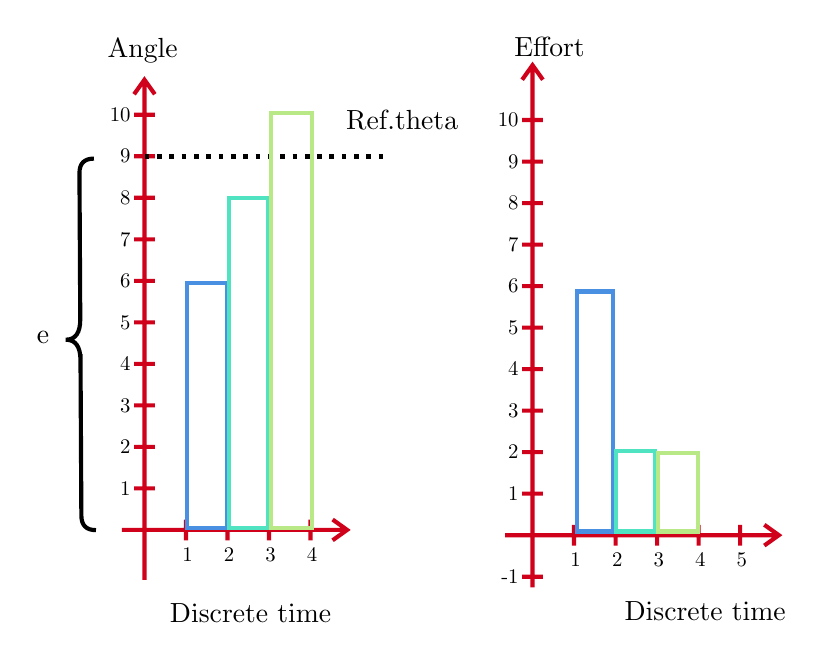
\begin{tikzpicture}[x=0.75pt,y=0.75pt,yscale=-1,xscale=1]
%uncomment if require: \path (0,530); %set diagram left start at 0, and has height of 530

%Shape: Axis 2D [id:dp9137510297707208] 
\draw [color={rgb, 255:red, 208; green, 2; blue, 27 }  ,draw opacity=1 ][line width=1.5]  (90,242.9) -- (198.5,242.9)(100.85,26) -- (100.85,267) (191.5,237.9) -- (198.5,242.9) -- (191.5,247.9) (95.85,33) -- (100.85,26) -- (105.85,33) (120.85,237.9) -- (120.85,247.9)(140.85,237.9) -- (140.85,247.9)(160.85,237.9) -- (160.85,247.9)(180.85,237.9) -- (180.85,247.9)(95.85,222.9) -- (105.85,222.9)(95.85,202.9) -- (105.85,202.9)(95.85,182.9) -- (105.85,182.9)(95.85,162.9) -- (105.85,162.9)(95.85,142.9) -- (105.85,142.9)(95.85,122.9) -- (105.85,122.9)(95.85,102.9) -- (105.85,102.9)(95.85,82.9) -- (105.85,82.9)(95.85,62.9) -- (105.85,62.9)(95.85,42.9) -- (105.85,42.9) ;
\draw   (127.85,254.9) node[anchor=east, scale=0.75]{1} (147.85,254.9) node[anchor=east, scale=0.75]{2} (167.85,254.9) node[anchor=east, scale=0.75]{3} (187.85,254.9) node[anchor=east, scale=0.75]{4} (97.85,222.9) node[anchor=east, scale=0.75]{1} (97.85,202.9) node[anchor=east, scale=0.75]{2} (97.85,182.9) node[anchor=east, scale=0.75]{3} (97.85,162.9) node[anchor=east, scale=0.75]{4} (97.85,142.9) node[anchor=east, scale=0.75]{5} (97.85,122.9) node[anchor=east, scale=0.75]{6} (97.85,102.9) node[anchor=east, scale=0.75]{7} (97.85,82.9) node[anchor=east, scale=0.75]{8} (97.85,62.9) node[anchor=east, scale=0.75]{9} (97.85,42.9) node[anchor=east, scale=0.75]{10} ;
%Straight Lines [id:da4351106715512081] 
\draw [line width=1.5]  [dash pattern={on 1.69pt off 2.76pt}]  (101,63) -- (218.5,63) ;


%Shape: Brace [id:dp994707289933978] 
\draw  [line width=1.5]  (76.5,64) .. controls (71.83,64.03) and (69.51,66.37) .. (69.54,71.04) -- (69.93,141.23) .. controls (69.97,147.9) and (67.66,151.24) .. (62.99,151.27) .. controls (67.66,151.24) and (70.01,154.56) .. (70.04,161.23)(70.03,158.23) -- (70.46,236.04) .. controls (70.49,240.71) and (72.83,243.03) .. (77.5,243) ;
%Shape: Rectangle [id:dp26090470643958286] 
\draw  [color={rgb, 255:red, 74; green, 144; blue, 226 }  ,draw opacity=1 ][line width=1.5]  (121.5,124) -- (140.5,124) -- (140.5,242) -- (121.5,242) -- cycle ;
%Shape: Rectangle [id:dp02841982011085853] 
\draw  [color={rgb, 255:red, 80; green, 227; blue, 194 }  ,draw opacity=1 ][line width=1.5]  (141.67,83) -- (160.5,83) -- (160.5,242) -- (141.67,242) -- cycle ;
%Shape: Rectangle [id:dp8528888145708966] 
\draw  [color={rgb, 255:red, 184; green, 233; blue, 134 }  ,draw opacity=1 ][line width=1.5]  (161.67,42) -- (181.67,42) -- (181.67,242) -- (161.67,242) -- cycle ;
%Shape: Axis 2D [id:dp5326952598948764] 
\draw [color={rgb, 255:red, 208; green, 2; blue, 27 }  ,draw opacity=1 ][line width=1.5]  (274.65,245.44) -- (406.5,245.44)(287.83,19) -- (287.83,270.6) (399.5,240.44) -- (406.5,245.44) -- (399.5,250.44) (282.83,26) -- (287.83,19) -- (292.83,26) (307.83,240.44) -- (307.83,250.44)(327.84,240.44) -- (327.84,250.44)(347.84,240.44) -- (347.84,250.44)(367.84,240.44) -- (367.84,250.44)(387.84,240.44) -- (387.84,250.44)(282.83,225.44) -- (292.83,225.44)(282.83,205.44) -- (292.83,205.44)(282.83,185.44) -- (292.83,185.44)(282.83,165.44) -- (292.83,165.44)(282.83,145.44) -- (292.83,145.44)(282.83,125.44) -- (292.83,125.44)(282.83,105.44) -- (292.83,105.44)(282.83,85.44) -- (292.83,85.44)(282.83,65.44) -- (292.83,65.44)(282.83,45.44) -- (292.83,45.44)(282.83,265.44) -- (292.83,265.44) ;
\draw   (314.83,257.44) node[anchor=east, scale=0.75]{1} (334.84,257.44) node[anchor=east, scale=0.75]{2} (354.84,257.44) node[anchor=east, scale=0.75]{3} (374.84,257.44) node[anchor=east, scale=0.75]{4} (394.84,257.44) node[anchor=east, scale=0.75]{5} (284.83,225.44) node[anchor=east, scale=0.75]{1} (284.83,205.44) node[anchor=east, scale=0.75]{2} (284.83,185.44) node[anchor=east, scale=0.75]{3} (284.83,165.44) node[anchor=east, scale=0.75]{4} (284.83,145.44) node[anchor=east, scale=0.75]{5} (284.83,125.44) node[anchor=east, scale=0.75]{6} (284.83,105.44) node[anchor=east, scale=0.75]{7} (284.83,85.44) node[anchor=east, scale=0.75]{8} (284.83,65.44) node[anchor=east, scale=0.75]{9} (284.83,45.44) node[anchor=east, scale=0.75]{10} (284.83,265.44) node[anchor=east, scale=0.75]{-1} ;
%Shape: Rectangle [id:dp37091810601651853] 
\draw  [color={rgb, 255:red, 74; green, 144; blue, 226 }  ,draw opacity=1 ][line width=1.5]  (309.42,128) -- (326.5,128) -- (326.5,243.67) -- (309.42,243.67) -- cycle ;
%Shape: Rectangle [id:dp5213748938493563] 
\draw  [color={rgb, 255:red, 80; green, 227; blue, 194 }  ,draw opacity=1 ][line width=1.5]  (328.08,205) -- (346.75,205) -- (346.75,243.67) -- (328.08,243.67) -- cycle ;
%Shape: Rectangle [id:dp3862836064219044] 
\draw  [color={rgb, 255:red, 184; green, 233; blue, 134 }  ,draw opacity=1 ][line width=1.5]  (348.08,206) -- (367.42,206) -- (367.42,243.67) -- (348.08,243.67) -- cycle ;

% Text Node
\draw (225,45.33) node  [align=left] {Ref.theta};
% Text Node
\draw (52,150) node  [align=left] {e};
% Text Node
\draw (100,12) node  [align=left] {Angle};
% Text Node
\draw (152,283) node  [align=left] {Discrete time};
% Text Node
\draw (296,10) node  [align=left] {Effort};
% Text Node
\draw (371,282) node  [align=left] {Discrete time};


\end{tikzpicture}
    \caption{A $K_D$ gain of 1 then only the rate of change in the error has and effect on the effort.}
    \label{fig:DGain}
\end{figure}

\paragraph{Discrete time} In the real world we live in a continues time domain, but computers works in discrete time domain. The discrete time is not measured in seconds, but rather in time frames.\\

On a note to a PID controller in theory, the perfect gains can be found, with the most suited rise time and settling time, but in practise this can be an expensive task. The expenses of the system can get high due to the need of a motor that is able to spin and stop at a rate that is suited for the PID controller, and sensors for the system needs to sense the changes within the system at the same rate.\\

\subsubsection{Dynamixel Servo PID}
In each Dynamixel servo there is an build in controller, that contains a feedback loop with an implemented PID controller with limiters to ensure that servos rotation velocity do not exceed a lower and an high threshold\cite{PIDmxx}. The feedback loop and the PID controller can be customised to fit the purpose of the objective.
\begin{figure}[H]
    \centering
    \includegraphics[width=\textwidth]{Figures/Technical_figures/PIDMX.PNG}
    \caption{Internal build in PID controller\cite{PIDmxx}}
    \label{fig:PIDMX}
\end{figure}

The servos positing and velocity is analysed through the use of an encoder, places on the gearing of the motor.  

\\

A short introduction to sEMG was given in the control systems section \ref{sEMG}. A more detailed description on how to make input control system from the sEMG can be found later in the report.

\paragraph{Electromyography} or EMG. as it has been called throughout this project, is a visualisation of the sum of difference in the potential measured fibres within one muscle. A skeletal muscle is made up of many small fibres called myofibril that each produces a difference in the potential. This signal needs amplification furthermore the signal has to be processed with the help of the analogue process, as described later in the section, in order to create a reliable source of control. The use of EMG is well documented in different articles in the use of a prosthetic arm  \cite{Castellini2009}. The EMG signal in this report is used to describe the signal that is being interpret.

\subsection*{Signal processing}
When the control unit receives the sEMG data, either through a micro-controller or a computer that processes the data, the data is the raw input data from the sEMG and cannot be used as an input for a control system. It is therefore clear that there is a need for processing the received data. In this project the signal is analysed through method of root mean square(RMS) which is an implemented part of the hardware, this is described later in this section.
\\ 

\subsubsection{Filters}
Digital filters is an important part of signal processing. 
These filters removes the noise in the signal depending on what frequencies of the signal that is useful for a robot or radio. A robot needs low frequencies due to it being a mechanical system.\\
Filters are classified as the frequency types it will filter on the signal. Two of the filters, the \textbf{low-pass} and the \textbf{high-pass} describes the filters that let the signal pass above or below a certain cutoff frequency. There is also the band-pass, and the band-stop filter which let the frequency's in a defined bandwidth pass through or block them respectively.
The most suited filter should be chosen based on analysis of the signal.

\paragraph{Sampling}
Certain precautions needs to be taken when sampling the sEMG signal. according to the \textit{Nyquist theorem} the sampling rate should be at least twice that of the signal frequency in order to insure the sinusoid of the EMG signal can be recreated. If this is not done then the data could be corrupted by the aliasing phenomenon. \cite{Nyquist}

%there are in general two use categorys, \textit{signal separation} and \textit{signal restoration}. \cite{FilterBa67:online}


%\paragraph{Signal separation} as the name implies this category seperates the signal passed through. this is normally used when the signal is contaminated with signal noise or other interference. in praxis an example could be a muscle sensor on the pectoralis major. here the signal might be contaminated with noise from the heart or other muscles. 
%therefore there would be a need to seperate the signals and isolate the wanted muscle signal.\cite{FilterBa67:online}
%\paragraph{signal restoration} this refers to when a signal has been distorted. an example could be an audio recording. after filtering it, the sound quality might improve beyond the original. \cite{FilterBa67:online}

\subsection*{Electronic hardware} \label{sec:elHW}
For a signal to be used in a software application there is a need for a way to interpret the signal. In this project the use of an EMG signal requires a hardware part, in this case, it is the muscle sensor v 3.0 from Advancer technology. The muscle sensor measures the signal through the electrodes placed on the user, furthermore, the device amplifies the signal by a gain of 100, it also rectifies the wave signal, which will be described later. The EMG sensor smooths the signal and convert it from an analogue signal to a digital signal that can be processed\cite{EMGHARD}.\\
As seen in figure: \ref{fig:GainsEMG}, the gain is decided through resistor R1, the voltage goes through MID and END, which are EMG inputs. The EMG signals then get amplified across the operational amplifier(OP AMP).\\

\begin{multicols}{2}  
\begin{figure}[H]
    \centering
    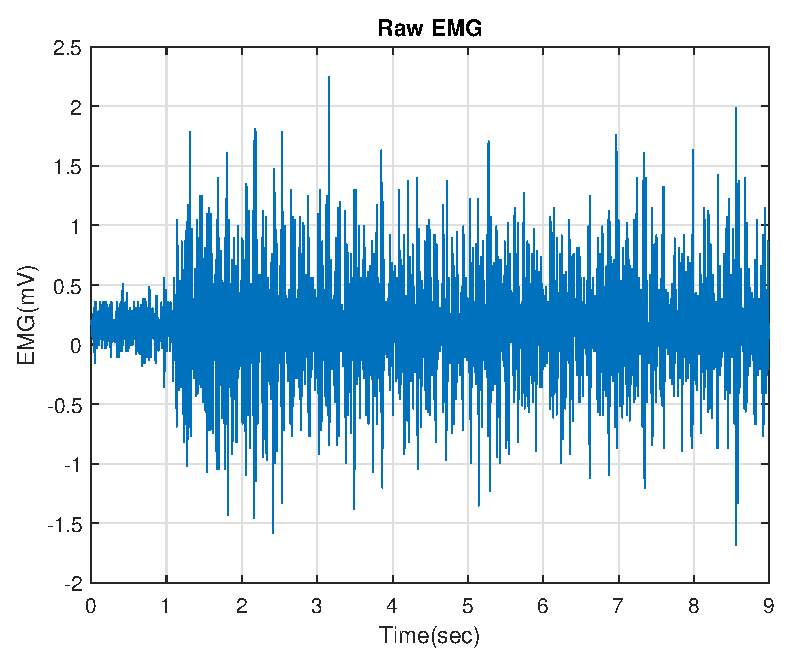
\includegraphics[width=0.4\textwidth]{Figures/EMG/epsFigRAW}
    \caption{\centering{EMG in a raw form analysed \\through matlab, data was borrow from\cite{EMGDATA}}}
\end{figure} 
\columnbreak
\begin{figure}[H]
    \centering
    \includegraphics[width=0.4\textwidth]{Figures/EMG/AmpGB.PNG}
    \caption{\centering{The schematics of the gain of the sEMG signal}\cite{SparkfunScematicEMG}}
    \label{fig:GainsEMG}
\end{figure} 
\end{multicols}

\paragraph{Full wave}
rectifying can be done by hardware or software. The software approach can be done simply by taking the absolute value  of the input data, in this case the hardware rectify the wave\cite{RMS}. Since the signal is an alternating waveform the signal is now only represented as positive numbers. Furthermore, the negative part of the data-set is conserved by squaring the value. This is important for the next step in analysing the data signal, and the root mean square process.\\
The schematics of rectifying the signal can be seen in \ref{fig:rect}, has a input from the latest schematic "Measure", where it polarises the input through a capacitor, and send the polarised signal through a 150k resistor. The signal is then sent through a serial connection, connected with junctions which includes known OP AMP's and ground inputs. The signal is now rectified.\\

\begin{multicols}{2}
\begin{figure}[H]
    \centering
   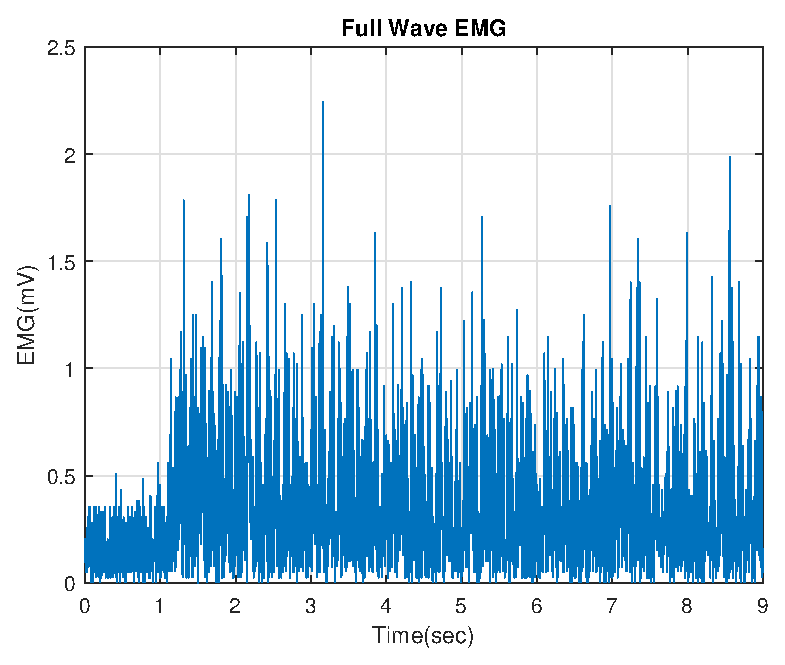
\includegraphics[width=0.3\textwidth]{Figures/EMG/epsFig}
    \caption{\centering{ EMG in Full wave form analysed \\through Matlab, data was borrow from \cite{EMGDATA}}}
\end{figure} 
\columnbreak
\begin{figure}[H]
    \centering
    \includegraphics[width=0.7\textwidth]{Figures/EMG/Rect.PNG}
    \caption{\centering{The schematics of the rectifying on the EMG sensors}\cite{SparkfunScematicEMG}}
    \label{fig:rect}
\end{figure} 
\end{multicols} 
\paragraph{Root mean square} or RMS is a solution made in order to get an average over time from any signal. It needs the wave form described in the full wave, this is referring to the squared part of RMS, so the means of the EMG signal can be evaluated, refraining from the rectifying of the squared part gets the mean of zero\cite{RMS}. After processing the signal it
is used as an implementation for a control signal.\\
The next step of schematics is as seen in \ref{fig:smooth}, is smoothing out the signal as described above. The rectified signal gets processed in a serial connection with known OP AMP's, resistors and capacitors. When the EMG signal is sent through this part of EMG sensor, the signal is smoothed.\\
The last schematics \ref{fig:finalGain}, with smooth signal as input, it is again put through a OP AMP to get the last gain before the signal is converted into a digital representation of the signal. The gain in this OP AMP is decided through the potentiometer.\\


\begin{multicols}{2}
\begin{figure}[H]
    \centering
    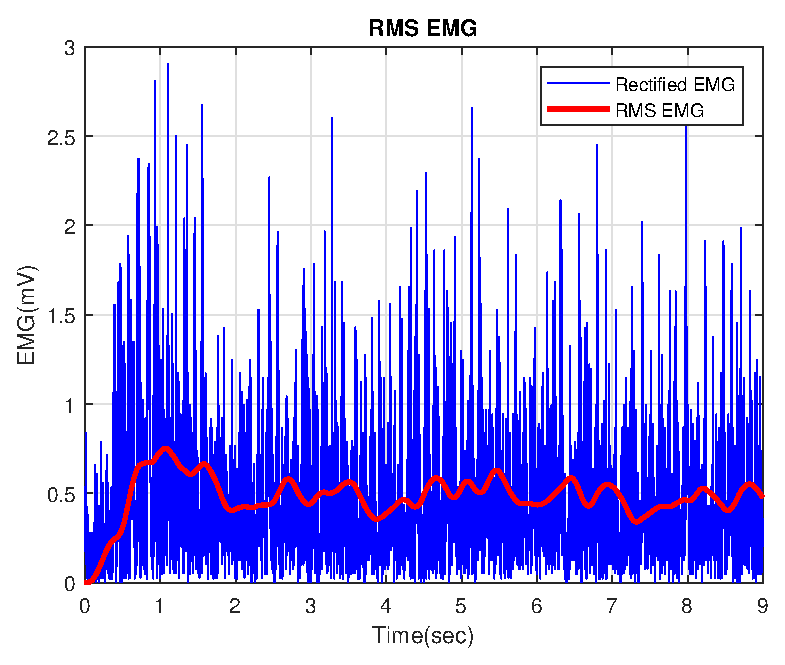
\includegraphics[width=0.4\textwidth]{Figures/EMG/epsFigRMS}
    \caption{EMG in Full wave with RMS analyses\\ preformed in matlab, data was borrow from\cite{EMGDATA}}
    \label{ref:Wasmooth}
\end{figure}
\columnbreak
\begin{figure}[H]
    \centering
    \includegraphics[width=0.4\textwidth]{Figures/EMG/Smooth.PNG}
    \caption{The schematics of the smoothing on the EMG sensors\cite{SparkfunScematicEMG}}
    \label{fig:smooth}
\end{figure} 
\end{multicols}




\begin{figure}[H]
    \centering
    \includegraphics[width=0.5\textwidth]{Figures/EMG/FinalGain.PNG}
    \caption{\centering{The schematics of the last gain on the EMG sensors before data is transmitted\cite{SparkfunScematicEMG}}}
    \label{fig:finalGain}
\end{figure} 


\subsection*{Muscle choice}
 Any distinct muscles which can voluntarily be controlled by the user could, in theory, be used as the input to the control system. Examples of possible choices could be the use of facial muscles, or the use of the muscles from the remaining arm. Surgically attaching the muscles closer to the skin to get a better signal is also an option \cite{SimonsSu49:online}.\\
 Difficulties in receiving a stable signal will change depending on the electrodes location on the body, e.g the breast muscles on the upper torso. The torso-muscles could be an ideal choice for some users, but if the electrodes were to be placed close to the heart, the heart-rhythm could interfere with the signal, while heightening the difficulties in receiving a stable control signal, due to the added noise from the heart, and would need to be filtered out. \\
 As a proof of concept the muscles in the lower arm as seen in figures \ref{ref:UpperArm} and \ref{fig:UnderArm} is used due to their accessible location when placing the electrodes while testing.
\begin{multicols}{2}
\begin{figure}[H]
    \centering
    \includegraphics[width=0.4\textwidth]{Figures/Technical_figures/OverArm.jpg}
    \caption{Picture showing the placement of electrodes on top of the forearm, where the green electrode is the neutral point, and both the black and red electrodes are placed on the same muscle}
    \label{ref:UpperArm}
\end{figure}
\columnbreak
\begin{figure}[H]
    \centering
    \includegraphics[width=0.4\textwidth]{Figures/Technical_figures/UnderArm.jpg}
    \caption{Figure showing the placement of electrodes under the forearm, where green is the neutral point, and both black and red is on the same muscle}
    \label{fig:UnderArm}
\end{figure} 
\end{multicols}


